% Created by tikzDevice version 0.10.1 on 2016-07-18 15:18:47
% !TEX encoding = UTF-8 Unicode
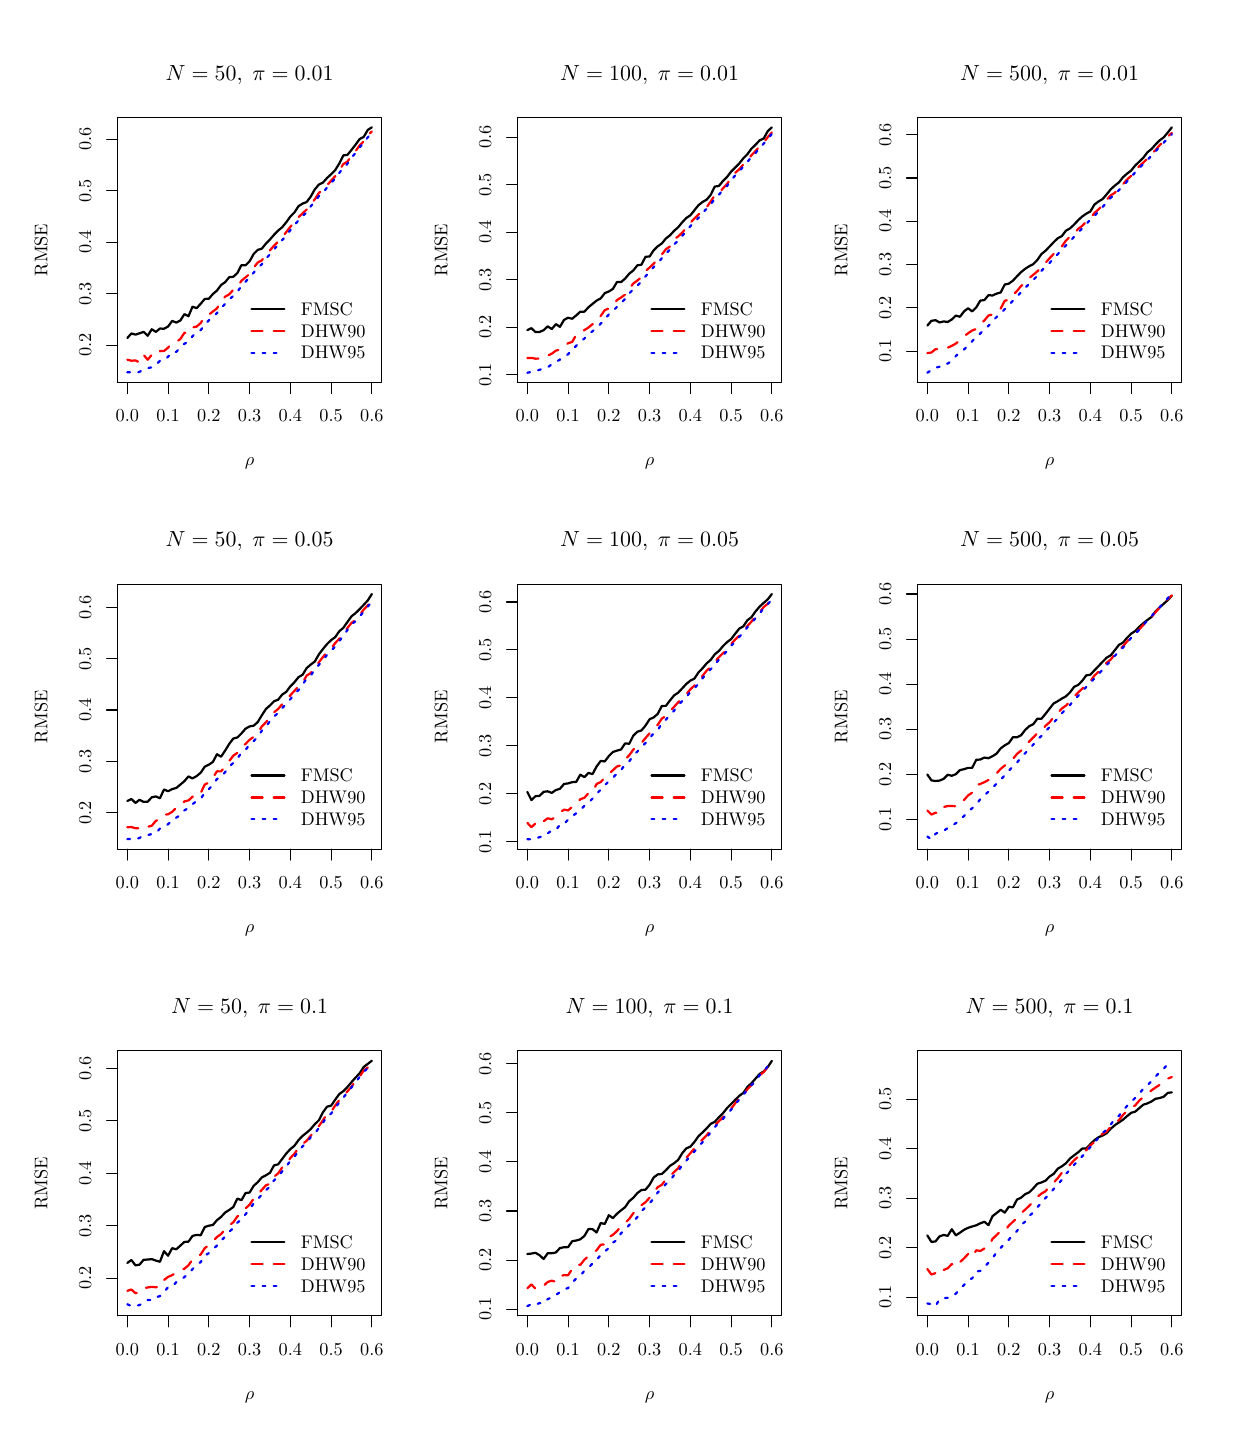
\begin{tikzpicture}[x=1pt,y=1pt]
\definecolor{fillColor}{RGB}{255,255,255}
\path[use as bounding box,fill=fillColor,fill opacity=0.00] (0,0) rectangle (433.62,505.89);
\begin{scope}
\path[clip] ( 32.47,377.65) rectangle (127.91,473.42);
\definecolor{drawColor}{RGB}{0,0,0}

\path[draw=drawColor,line width= 0.8pt,line join=round,line cap=round] ( 36.01,393.74) --
	( 37.48,395.40) --
	( 38.95,394.97) --
	( 40.42,395.45) --
	( 41.90,395.97) --
	( 43.37,394.55) --
	( 44.84,396.91) --
	( 46.32,395.96) --
	( 47.79,397.17) --
	( 49.26,397.09) --
	( 50.73,397.89) --
	( 52.21,399.93) --
	( 53.68,399.33) --
	( 55.15,400.04) --
	( 56.63,402.37) --
	( 58.10,401.61) --
	( 59.57,405.09) --
	( 61.04,404.51) --
	( 62.52,406.13) --
	( 63.99,407.86) --
	( 65.46,407.95) --
	( 66.93,409.64) --
	( 68.41,410.90) --
	( 69.88,412.90) --
	( 71.35,413.91) --
	( 72.83,415.74) --
	( 74.30,415.87) --
	( 75.77,417.22) --
	( 77.24,420.08) --
	( 78.72,420.02) --
	( 80.19,421.48) --
	( 81.66,424.11) --
	( 83.14,425.59) --
	( 84.61,426.04) --
	( 86.08,427.85) --
	( 87.55,429.35) --
	( 89.03,431.06) --
	( 90.50,432.55) --
	( 91.97,433.78) --
	( 93.44,435.57) --
	( 94.92,437.65) --
	( 96.39,439.12) --
	( 97.86,441.37) --
	( 99.34,442.32) --
	(100.81,442.88) --
	(102.28,444.83) --
	(103.75,447.45) --
	(105.23,449.19) --
	(106.70,449.92) --
	(108.17,451.56) --
	(109.65,452.92) --
	(111.12,454.41) --
	(112.59,456.80) --
	(114.06,459.74) --
	(115.54,459.92) --
	(117.01,461.72) --
	(118.48,463.61) --
	(119.95,465.63) --
	(121.43,466.42) --
	(122.90,468.94) --
	(124.37,469.87);
\end{scope}
\begin{scope}
\path[clip] (  0.00,  0.00) rectangle (433.62,505.89);
\definecolor{drawColor}{RGB}{0,0,0}

\path[draw=drawColor,line width= 0.4pt,line join=round,line cap=round] ( 36.01,377.65) -- (124.37,377.65);

\path[draw=drawColor,line width= 0.4pt,line join=round,line cap=round] ( 36.01,377.65) -- ( 36.01,373.69);

\path[draw=drawColor,line width= 0.4pt,line join=round,line cap=round] ( 50.73,377.65) -- ( 50.73,373.69);

\path[draw=drawColor,line width= 0.4pt,line join=round,line cap=round] ( 65.46,377.65) -- ( 65.46,373.69);

\path[draw=drawColor,line width= 0.4pt,line join=round,line cap=round] ( 80.19,377.65) -- ( 80.19,373.69);

\path[draw=drawColor,line width= 0.4pt,line join=round,line cap=round] ( 94.92,377.65) -- ( 94.92,373.69);

\path[draw=drawColor,line width= 0.4pt,line join=round,line cap=round] (109.65,377.65) -- (109.65,373.69);

\path[draw=drawColor,line width= 0.4pt,line join=round,line cap=round] (124.37,377.65) -- (124.37,373.69);

\node[text=drawColor,anchor=base,inner sep=0pt, outer sep=0pt, scale=  0.66] at ( 36.01,363.40) {0.0};

\node[text=drawColor,anchor=base,inner sep=0pt, outer sep=0pt, scale=  0.66] at ( 50.73,363.40) {0.1};

\node[text=drawColor,anchor=base,inner sep=0pt, outer sep=0pt, scale=  0.66] at ( 65.46,363.40) {0.2};

\node[text=drawColor,anchor=base,inner sep=0pt, outer sep=0pt, scale=  0.66] at ( 80.19,363.40) {0.3};

\node[text=drawColor,anchor=base,inner sep=0pt, outer sep=0pt, scale=  0.66] at ( 94.92,363.40) {0.4};

\node[text=drawColor,anchor=base,inner sep=0pt, outer sep=0pt, scale=  0.66] at (109.65,363.40) {0.5};

\node[text=drawColor,anchor=base,inner sep=0pt, outer sep=0pt, scale=  0.66] at (124.37,363.40) {0.6};

\path[draw=drawColor,line width= 0.4pt,line join=round,line cap=round] ( 32.47,391.13) -- ( 32.47,465.58);

\path[draw=drawColor,line width= 0.4pt,line join=round,line cap=round] ( 32.47,391.13) -- ( 28.51,391.13);

\path[draw=drawColor,line width= 0.4pt,line join=round,line cap=round] ( 32.47,409.74) -- ( 28.51,409.74);

\path[draw=drawColor,line width= 0.4pt,line join=round,line cap=round] ( 32.47,428.36) -- ( 28.51,428.36);

\path[draw=drawColor,line width= 0.4pt,line join=round,line cap=round] ( 32.47,446.97) -- ( 28.51,446.97);

\path[draw=drawColor,line width= 0.4pt,line join=round,line cap=round] ( 32.47,465.58) -- ( 28.51,465.58);

\node[text=drawColor,rotate= 90.00,anchor=base,inner sep=0pt, outer sep=0pt, scale=  0.66] at ( 22.97,391.13) {0.2};

\node[text=drawColor,rotate= 90.00,anchor=base,inner sep=0pt, outer sep=0pt, scale=  0.66] at ( 22.97,409.74) {0.3};

\node[text=drawColor,rotate= 90.00,anchor=base,inner sep=0pt, outer sep=0pt, scale=  0.66] at ( 22.97,428.36) {0.4};

\node[text=drawColor,rotate= 90.00,anchor=base,inner sep=0pt, outer sep=0pt, scale=  0.66] at ( 22.97,446.97) {0.5};

\node[text=drawColor,rotate= 90.00,anchor=base,inner sep=0pt, outer sep=0pt, scale=  0.66] at ( 22.97,465.58) {0.6};

\path[draw=drawColor,line width= 0.4pt,line join=round,line cap=round] ( 32.47,377.65) --
	(127.91,377.65) --
	(127.91,473.42) --
	( 32.47,473.42) --
	( 32.47,377.65);
\end{scope}
\begin{scope}
\path[clip] (  0.00,337.26) rectangle (144.54,505.89);
\definecolor{drawColor}{RGB}{0,0,0}

\node[text=drawColor,anchor=base,inner sep=0pt, outer sep=0pt, scale=  0.79] at ( 80.19,486.92) {\bfseries $N=50, \;\pi=0.01$};

\node[text=drawColor,anchor=base,inner sep=0pt, outer sep=0pt, scale=  0.66] at ( 80.19,347.56) {$\rho$};

\node[text=drawColor,rotate= 90.00,anchor=base,inner sep=0pt, outer sep=0pt, scale=  0.66] at (  7.13,425.53) {RMSE};
\end{scope}
\begin{scope}
\path[clip] ( 32.47,377.65) rectangle (127.91,473.42);
\definecolor{drawColor}{RGB}{255,0,0}

\path[draw=drawColor,line width= 0.8pt,dash pattern=on 4pt off 4pt ,line join=round,line cap=round] ( 36.01,385.91) --
	( 37.48,385.53) --
	( 38.95,385.65) --
	( 40.42,384.94) --
	( 41.90,387.63) --
	( 43.37,385.90) --
	( 44.84,387.68) --
	( 46.32,387.28) --
	( 47.79,388.99) --
	( 49.26,389.07) --
	( 50.73,390.26) --
	( 52.21,391.84) --
	( 53.68,392.34) --
	( 55.15,393.35) --
	( 56.63,395.63) --
	( 58.10,395.52) --
	( 59.57,397.57) --
	( 61.04,397.86) --
	( 62.52,399.15) --
	( 63.99,401.53) --
	( 65.46,402.16) --
	( 66.93,403.33) --
	( 68.41,404.45) --
	( 69.88,407.08) --
	( 71.35,408.69) --
	( 72.83,409.52) --
	( 74.30,411.16) --
	( 75.77,412.10) --
	( 77.24,414.45) --
	( 78.72,415.62) --
	( 80.19,417.00) --
	( 81.66,419.18) --
	( 83.14,421.03) --
	( 84.61,421.79) --
	( 86.08,423.83) --
	( 87.55,425.44) --
	( 89.03,427.14) --
	( 90.50,428.55) --
	( 91.97,430.23) --
	( 93.44,432.03) --
	( 94.92,433.91) --
	( 96.39,435.59) --
	( 97.86,437.42) --
	( 99.34,438.79) --
	(100.81,440.17) --
	(102.28,442.23) --
	(103.75,443.84) --
	(105.23,446.17) --
	(106.70,447.36) --
	(108.17,448.87) --
	(109.65,450.62) --
	(111.12,452.18) --
	(112.59,454.28) --
	(114.06,456.61) --
	(115.54,457.49) --
	(117.01,459.55) --
	(118.48,461.28) --
	(119.95,463.36) --
	(121.43,464.77) --
	(122.90,466.97) --
	(124.37,468.41);
\definecolor{drawColor}{RGB}{0,0,255}

\path[draw=drawColor,line width= 0.8pt,dash pattern=on 1pt off 3pt ,line join=round,line cap=round] ( 36.01,381.38) --
	( 37.48,381.38) --
	( 38.95,381.20) --
	( 40.42,381.51) --
	( 41.90,382.38) --
	( 43.37,382.84) --
	( 44.84,383.16) --
	( 46.32,384.09) --
	( 47.79,385.47) --
	( 49.26,385.60) --
	( 50.73,387.01) --
	( 52.21,388.68) --
	( 53.68,388.74) --
	( 55.15,390.23) --
	( 56.63,391.66) --
	( 58.10,392.47) --
	( 59.57,394.39) --
	( 61.04,395.76) --
	( 62.52,396.60) --
	( 63.99,398.48) --
	( 65.46,400.14) --
	( 66.93,401.26) --
	( 68.41,402.79) --
	( 69.88,404.52) --
	( 71.35,406.09) --
	( 72.83,407.67) --
	( 74.30,408.97) --
	( 75.77,410.47) --
	( 77.24,412.52) --
	( 78.72,414.08) --
	( 80.19,415.67) --
	( 81.66,417.36) --
	( 83.14,419.03) --
	( 84.61,420.38) --
	( 86.08,422.46) --
	( 87.55,423.98) --
	( 89.03,425.82) --
	( 90.50,427.43) --
	( 91.97,429.12) --
	( 93.44,430.72) --
	( 94.92,432.75) --
	( 96.39,434.57) --
	( 97.86,436.21) --
	( 99.34,437.83) --
	(100.81,439.14) --
	(102.28,441.33) --
	(103.75,443.07) --
	(105.23,444.99) --
	(106.70,446.21) --
	(108.17,448.13) --
	(109.65,449.73) --
	(111.12,451.45) --
	(112.59,453.39) --
	(114.06,455.21) --
	(115.54,456.71) --
	(117.01,458.95) --
	(118.48,460.55) --
	(119.95,462.61) --
	(121.43,464.24) --
	(122.90,466.26) --
	(124.37,467.81);
\definecolor{drawColor}{RGB}{0,0,0}

\path[draw=drawColor,line width= 0.8pt,line join=round,line cap=round] ( 80.89,404.28) -- ( 92.77,404.28);
\definecolor{drawColor}{RGB}{255,0,0}

\path[draw=drawColor,line width= 0.8pt,dash pattern=on 4pt off 4pt ,line join=round,line cap=round] ( 80.89,396.36) -- ( 92.77,396.36);
\definecolor{drawColor}{RGB}{0,0,255}

\path[draw=drawColor,line width= 0.8pt,dash pattern=on 1pt off 3pt ,line join=round,line cap=round] ( 80.89,388.44) -- ( 92.77,388.44);
\definecolor{drawColor}{RGB}{0,0,0}

\node[text=drawColor,anchor=base west,inner sep=0pt, outer sep=0pt, scale=  0.66] at ( 98.71,402.01) {FMSC};

\node[text=drawColor,anchor=base west,inner sep=0pt, outer sep=0pt, scale=  0.66] at ( 98.71,394.09) {DHW90};

\node[text=drawColor,anchor=base west,inner sep=0pt, outer sep=0pt, scale=  0.66] at ( 98.71,386.17) {DHW95};
\end{scope}
\begin{scope}
\path[clip] (177.01,377.65) rectangle (272.45,473.42);
\definecolor{drawColor}{RGB}{0,0,0}

\path[draw=drawColor,line width= 0.8pt,line join=round,line cap=round] (180.55,396.61) --
	(182.02,397.30) --
	(183.49,395.89) --
	(184.96,395.91) --
	(186.44,396.59) --
	(187.91,397.95) --
	(189.38,396.98) --
	(190.86,398.75) --
	(192.33,397.77) --
	(193.80,400.28) --
	(195.27,401.07) --
	(196.75,400.70) --
	(198.22,401.92) --
	(199.69,403.26) --
	(201.17,403.27) --
	(202.64,404.85) --
	(204.11,406.08) --
	(205.58,407.26) --
	(207.06,408.06) --
	(208.53,409.96) --
	(210.00,410.55) --
	(211.47,411.50) --
	(212.95,413.99) --
	(214.42,413.95) --
	(215.89,415.22) --
	(217.37,416.99) --
	(218.84,418.15) --
	(220.31,420.00) --
	(221.78,420.24) --
	(223.26,423.11) --
	(224.73,423.19) --
	(226.20,425.44) --
	(227.68,426.90) --
	(229.15,427.89) --
	(230.62,429.71) --
	(232.09,430.84) --
	(233.57,432.46) --
	(235.04,433.75) --
	(236.51,435.53) --
	(237.98,437.10) --
	(239.46,438.07) --
	(240.93,439.91) --
	(242.40,441.75) --
	(243.88,442.91) --
	(245.35,443.73) --
	(246.82,445.49) --
	(248.29,448.48) --
	(249.77,448.68) --
	(251.24,450.48) --
	(252.71,451.94) --
	(254.19,453.87) --
	(255.66,455.35) --
	(257.13,456.82) --
	(258.60,458.69) --
	(260.08,460.17) --
	(261.55,462.18) --
	(263.02,463.58) --
	(264.50,465.17) --
	(265.97,465.85) --
	(267.44,468.50) --
	(268.91,469.87);
\end{scope}
\begin{scope}
\path[clip] (  0.00,  0.00) rectangle (433.62,505.89);
\definecolor{drawColor}{RGB}{0,0,0}

\path[draw=drawColor,line width= 0.4pt,line join=round,line cap=round] (180.55,377.65) -- (268.91,377.65);

\path[draw=drawColor,line width= 0.4pt,line join=round,line cap=round] (180.55,377.65) -- (180.55,373.69);

\path[draw=drawColor,line width= 0.4pt,line join=round,line cap=round] (195.27,377.65) -- (195.27,373.69);

\path[draw=drawColor,line width= 0.4pt,line join=round,line cap=round] (210.00,377.65) -- (210.00,373.69);

\path[draw=drawColor,line width= 0.4pt,line join=round,line cap=round] (224.73,377.65) -- (224.73,373.69);

\path[draw=drawColor,line width= 0.4pt,line join=round,line cap=round] (239.46,377.65) -- (239.46,373.69);

\path[draw=drawColor,line width= 0.4pt,line join=round,line cap=round] (254.19,377.65) -- (254.19,373.69);

\path[draw=drawColor,line width= 0.4pt,line join=round,line cap=round] (268.91,377.65) -- (268.91,373.69);

\node[text=drawColor,anchor=base,inner sep=0pt, outer sep=0pt, scale=  0.66] at (180.55,363.40) {0.0};

\node[text=drawColor,anchor=base,inner sep=0pt, outer sep=0pt, scale=  0.66] at (195.27,363.40) {0.1};

\node[text=drawColor,anchor=base,inner sep=0pt, outer sep=0pt, scale=  0.66] at (210.00,363.40) {0.2};

\node[text=drawColor,anchor=base,inner sep=0pt, outer sep=0pt, scale=  0.66] at (224.73,363.40) {0.3};

\node[text=drawColor,anchor=base,inner sep=0pt, outer sep=0pt, scale=  0.66] at (239.46,363.40) {0.4};

\node[text=drawColor,anchor=base,inner sep=0pt, outer sep=0pt, scale=  0.66] at (254.19,363.40) {0.5};

\node[text=drawColor,anchor=base,inner sep=0pt, outer sep=0pt, scale=  0.66] at (268.91,363.40) {0.6};

\path[draw=drawColor,line width= 0.4pt,line join=round,line cap=round] (177.01,380.55) -- (177.01,466.31);

\path[draw=drawColor,line width= 0.4pt,line join=round,line cap=round] (177.01,380.55) -- (173.05,380.55);

\path[draw=drawColor,line width= 0.4pt,line join=round,line cap=round] (177.01,397.70) -- (173.05,397.70);

\path[draw=drawColor,line width= 0.4pt,line join=round,line cap=round] (177.01,414.85) -- (173.05,414.85);

\path[draw=drawColor,line width= 0.4pt,line join=round,line cap=round] (177.01,432.01) -- (173.05,432.01);

\path[draw=drawColor,line width= 0.4pt,line join=round,line cap=round] (177.01,449.16) -- (173.05,449.16);

\path[draw=drawColor,line width= 0.4pt,line join=round,line cap=round] (177.01,466.31) -- (173.05,466.31);

\node[text=drawColor,rotate= 90.00,anchor=base,inner sep=0pt, outer sep=0pt, scale=  0.66] at (167.51,380.55) {0.1};

\node[text=drawColor,rotate= 90.00,anchor=base,inner sep=0pt, outer sep=0pt, scale=  0.66] at (167.51,397.70) {0.2};

\node[text=drawColor,rotate= 90.00,anchor=base,inner sep=0pt, outer sep=0pt, scale=  0.66] at (167.51,414.85) {0.3};

\node[text=drawColor,rotate= 90.00,anchor=base,inner sep=0pt, outer sep=0pt, scale=  0.66] at (167.51,432.01) {0.4};

\node[text=drawColor,rotate= 90.00,anchor=base,inner sep=0pt, outer sep=0pt, scale=  0.66] at (167.51,449.16) {0.5};

\node[text=drawColor,rotate= 90.00,anchor=base,inner sep=0pt, outer sep=0pt, scale=  0.66] at (167.51,466.31) {0.6};

\path[draw=drawColor,line width= 0.4pt,line join=round,line cap=round] (177.01,377.65) --
	(272.45,377.65) --
	(272.45,473.42) --
	(177.01,473.42) --
	(177.01,377.65);
\end{scope}
\begin{scope}
\path[clip] (144.54,337.26) rectangle (289.08,505.89);
\definecolor{drawColor}{RGB}{0,0,0}

\node[text=drawColor,anchor=base,inner sep=0pt, outer sep=0pt, scale=  0.79] at (224.73,486.92) {\bfseries $N=100, \;\pi=0.01$};

\node[text=drawColor,anchor=base,inner sep=0pt, outer sep=0pt, scale=  0.66] at (224.73,347.56) {$\rho$};

\node[text=drawColor,rotate= 90.00,anchor=base,inner sep=0pt, outer sep=0pt, scale=  0.66] at (151.67,425.53) {RMSE};
\end{scope}
\begin{scope}
\path[clip] (177.01,377.65) rectangle (272.45,473.42);
\definecolor{drawColor}{RGB}{255,0,0}

\path[draw=drawColor,line width= 0.8pt,dash pattern=on 4pt off 4pt ,line join=round,line cap=round] (180.55,386.51) --
	(182.02,386.56) --
	(183.49,386.28) --
	(184.96,386.32) --
	(186.44,387.09) --
	(187.91,387.34) --
	(189.38,388.08) --
	(190.86,389.18) --
	(192.33,389.58) --
	(193.80,390.84) --
	(195.27,391.85) --
	(196.75,392.34) --
	(198.22,394.89) --
	(199.69,395.78) --
	(201.17,396.60) --
	(202.64,397.54) --
	(204.11,398.73) --
	(205.58,400.58) --
	(207.06,401.70) --
	(208.53,403.81) --
	(210.00,404.42) --
	(211.47,405.54) --
	(212.95,407.46) --
	(214.42,408.39) --
	(215.89,409.43) --
	(217.37,411.43) --
	(218.84,413.45) --
	(220.31,414.52) --
	(221.78,415.72) --
	(223.26,417.94) --
	(224.73,419.23) --
	(226.20,420.60) --
	(227.68,422.34) --
	(229.15,423.91) --
	(230.62,425.84) --
	(232.09,426.83) --
	(233.57,429.46) --
	(235.04,430.43) --
	(236.51,431.81) --
	(237.98,433.57) --
	(239.46,435.38) --
	(240.93,436.95) --
	(242.40,438.35) --
	(243.88,439.90) --
	(245.35,441.02) --
	(246.82,443.07) --
	(248.29,445.35) --
	(249.77,446.08) --
	(251.24,447.82) --
	(252.71,449.41) --
	(254.19,451.55) --
	(255.66,453.45) --
	(257.13,454.71) --
	(258.60,456.47) --
	(260.08,457.96) --
	(261.55,459.80) --
	(263.02,461.33) --
	(264.50,462.92) --
	(265.97,464.43) --
	(267.44,466.36) --
	(268.91,468.02);
\definecolor{drawColor}{RGB}{0,0,255}

\path[draw=drawColor,line width= 0.8pt,dash pattern=on 1pt off 3pt ,line join=round,line cap=round] (180.55,381.20) --
	(182.02,381.50) --
	(183.49,381.89) --
	(184.96,382.24) --
	(186.44,382.83) --
	(187.91,383.19) --
	(189.38,384.19) --
	(190.86,385.05) --
	(192.33,385.96) --
	(193.80,387.07) --
	(195.27,387.86) --
	(196.75,389.52) --
	(198.22,390.94) --
	(199.69,392.37) --
	(201.17,393.56) --
	(202.64,395.09) --
	(204.11,396.19) --
	(205.58,397.52) --
	(207.06,398.92) --
	(208.53,400.58) --
	(210.00,402.23) --
	(211.47,403.53) --
	(212.95,405.00) --
	(214.42,406.23) --
	(215.89,407.94) --
	(217.37,409.83) --
	(218.84,411.35) --
	(220.31,412.71) --
	(221.78,414.11) --
	(223.26,416.04) --
	(224.73,417.78) --
	(226.20,419.35) --
	(227.68,420.84) --
	(229.15,422.56) --
	(230.62,424.30) --
	(232.09,425.65) --
	(233.57,427.60) --
	(235.04,428.84) --
	(236.51,430.66) --
	(237.98,432.30) --
	(239.46,434.15) --
	(240.93,435.71) --
	(242.40,437.15) --
	(243.88,439.04) --
	(245.35,440.48) --
	(246.82,441.96) --
	(248.29,444.13) --
	(249.77,445.52) --
	(251.24,447.23) --
	(252.71,448.69) --
	(254.19,450.70) --
	(255.66,452.51) --
	(257.13,453.87) --
	(258.60,455.79) --
	(260.08,457.33) --
	(261.55,459.28) --
	(263.02,460.60) --
	(264.50,462.41) --
	(265.97,464.00) --
	(267.44,465.66) --
	(268.91,467.49);
\definecolor{drawColor}{RGB}{0,0,0}

\path[draw=drawColor,line width= 0.8pt,line join=round,line cap=round] (225.43,404.28) -- (237.31,404.28);
\definecolor{drawColor}{RGB}{255,0,0}

\path[draw=drawColor,line width= 0.8pt,dash pattern=on 4pt off 4pt ,line join=round,line cap=round] (225.43,396.36) -- (237.31,396.36);
\definecolor{drawColor}{RGB}{0,0,255}

\path[draw=drawColor,line width= 0.8pt,dash pattern=on 1pt off 3pt ,line join=round,line cap=round] (225.43,388.44) -- (237.31,388.44);
\definecolor{drawColor}{RGB}{0,0,0}

\node[text=drawColor,anchor=base west,inner sep=0pt, outer sep=0pt, scale=  0.66] at (243.25,402.01) {FMSC};

\node[text=drawColor,anchor=base west,inner sep=0pt, outer sep=0pt, scale=  0.66] at (243.25,394.09) {DHW90};

\node[text=drawColor,anchor=base west,inner sep=0pt, outer sep=0pt, scale=  0.66] at (243.25,386.17) {DHW95};
\end{scope}
\begin{scope}
\path[clip] (321.55,377.65) rectangle (416.99,473.42);
\definecolor{drawColor}{RGB}{0,0,0}

\path[draw=drawColor,line width= 0.8pt,line join=round,line cap=round] (325.09,398.24) --
	(326.56,399.95) --
	(328.03,400.18) --
	(329.50,399.37) --
	(330.98,399.73) --
	(332.45,399.55) --
	(333.92,400.43) --
	(335.40,401.85) --
	(336.87,401.41) --
	(338.34,403.35) --
	(339.81,404.50) --
	(341.29,403.36) --
	(342.76,404.79) --
	(344.23,407.27) --
	(345.71,407.45) --
	(347.18,409.22) --
	(348.65,409.11) --
	(350.12,409.79) --
	(351.60,410.21) --
	(353.07,413.07) --
	(354.54,413.40) --
	(356.01,414.46) --
	(357.49,416.06) --
	(358.96,417.56) --
	(360.43,418.74) --
	(361.91,419.69) --
	(363.38,420.44) --
	(364.85,421.96) --
	(366.32,424.08) --
	(367.80,425.28) --
	(369.27,426.81) --
	(370.74,428.37) --
	(372.22,429.79) --
	(373.69,430.56) --
	(375.16,432.52) --
	(376.63,433.35) --
	(378.11,434.72) --
	(379.58,436.31) --
	(381.05,437.65) --
	(382.52,438.67) --
	(384.00,439.47) --
	(385.47,441.97) --
	(386.94,443.08) --
	(388.42,443.95) --
	(389.89,445.65) --
	(391.36,447.48) --
	(392.83,448.81) --
	(394.31,449.96) --
	(395.78,451.83) --
	(397.25,453.13) --
	(398.73,454.24) --
	(400.20,456.09) --
	(401.67,457.46) --
	(403.14,458.88) --
	(404.62,460.86) --
	(406.09,462.02) --
	(407.56,463.68) --
	(409.04,465.18) --
	(410.51,466.24) --
	(411.98,468.01) --
	(413.45,469.87);
\end{scope}
\begin{scope}
\path[clip] (  0.00,  0.00) rectangle (433.62,505.89);
\definecolor{drawColor}{RGB}{0,0,0}

\path[draw=drawColor,line width= 0.4pt,line join=round,line cap=round] (325.09,377.65) -- (413.45,377.65);

\path[draw=drawColor,line width= 0.4pt,line join=round,line cap=round] (325.09,377.65) -- (325.09,373.69);

\path[draw=drawColor,line width= 0.4pt,line join=round,line cap=round] (339.81,377.65) -- (339.81,373.69);

\path[draw=drawColor,line width= 0.4pt,line join=round,line cap=round] (354.54,377.65) -- (354.54,373.69);

\path[draw=drawColor,line width= 0.4pt,line join=round,line cap=round] (369.27,377.65) -- (369.27,373.69);

\path[draw=drawColor,line width= 0.4pt,line join=round,line cap=round] (384.00,377.65) -- (384.00,373.69);

\path[draw=drawColor,line width= 0.4pt,line join=round,line cap=round] (398.73,377.65) -- (398.73,373.69);

\path[draw=drawColor,line width= 0.4pt,line join=round,line cap=round] (413.45,377.65) -- (413.45,373.69);

\node[text=drawColor,anchor=base,inner sep=0pt, outer sep=0pt, scale=  0.66] at (325.09,363.40) {0.0};

\node[text=drawColor,anchor=base,inner sep=0pt, outer sep=0pt, scale=  0.66] at (339.81,363.40) {0.1};

\node[text=drawColor,anchor=base,inner sep=0pt, outer sep=0pt, scale=  0.66] at (354.54,363.40) {0.2};

\node[text=drawColor,anchor=base,inner sep=0pt, outer sep=0pt, scale=  0.66] at (369.27,363.40) {0.3};

\node[text=drawColor,anchor=base,inner sep=0pt, outer sep=0pt, scale=  0.66] at (384.00,363.40) {0.4};

\node[text=drawColor,anchor=base,inner sep=0pt, outer sep=0pt, scale=  0.66] at (398.73,363.40) {0.5};

\node[text=drawColor,anchor=base,inner sep=0pt, outer sep=0pt, scale=  0.66] at (413.45,363.40) {0.6};

\path[draw=drawColor,line width= 0.4pt,line join=round,line cap=round] (321.55,389.03) -- (321.55,467.21);

\path[draw=drawColor,line width= 0.4pt,line join=round,line cap=round] (321.55,389.03) -- (317.59,389.03);

\path[draw=drawColor,line width= 0.4pt,line join=round,line cap=round] (321.55,404.67) -- (317.59,404.67);

\path[draw=drawColor,line width= 0.4pt,line join=round,line cap=round] (321.55,420.30) -- (317.59,420.30);

\path[draw=drawColor,line width= 0.4pt,line join=round,line cap=round] (321.55,435.94) -- (317.59,435.94);

\path[draw=drawColor,line width= 0.4pt,line join=round,line cap=round] (321.55,451.58) -- (317.59,451.58);

\path[draw=drawColor,line width= 0.4pt,line join=round,line cap=round] (321.55,467.21) -- (317.59,467.21);

\node[text=drawColor,rotate= 90.00,anchor=base,inner sep=0pt, outer sep=0pt, scale=  0.66] at (312.05,389.03) {0.1};

\node[text=drawColor,rotate= 90.00,anchor=base,inner sep=0pt, outer sep=0pt, scale=  0.66] at (312.05,404.67) {0.2};

\node[text=drawColor,rotate= 90.00,anchor=base,inner sep=0pt, outer sep=0pt, scale=  0.66] at (312.05,420.30) {0.3};

\node[text=drawColor,rotate= 90.00,anchor=base,inner sep=0pt, outer sep=0pt, scale=  0.66] at (312.05,435.94) {0.4};

\node[text=drawColor,rotate= 90.00,anchor=base,inner sep=0pt, outer sep=0pt, scale=  0.66] at (312.05,451.58) {0.5};

\node[text=drawColor,rotate= 90.00,anchor=base,inner sep=0pt, outer sep=0pt, scale=  0.66] at (312.05,467.21) {0.6};

\path[draw=drawColor,line width= 0.4pt,line join=round,line cap=round] (321.55,377.65) --
	(416.99,377.65) --
	(416.99,473.42) --
	(321.55,473.42) --
	(321.55,377.65);
\end{scope}
\begin{scope}
\path[clip] (289.08,337.26) rectangle (433.62,505.89);
\definecolor{drawColor}{RGB}{0,0,0}

\node[text=drawColor,anchor=base,inner sep=0pt, outer sep=0pt, scale=  0.79] at (369.27,486.92) {\bfseries $N=500, \;\pi=0.01$};

\node[text=drawColor,anchor=base,inner sep=0pt, outer sep=0pt, scale=  0.66] at (369.27,347.56) {$\rho$};

\node[text=drawColor,rotate= 90.00,anchor=base,inner sep=0pt, outer sep=0pt, scale=  0.66] at (296.21,425.53) {RMSE};
\end{scope}
\begin{scope}
\path[clip] (321.55,377.65) rectangle (416.99,473.42);
\definecolor{drawColor}{RGB}{255,0,0}

\path[draw=drawColor,line width= 0.8pt,dash pattern=on 4pt off 4pt ,line join=round,line cap=round] (325.09,388.31) --
	(326.56,388.49) --
	(328.03,389.72) --
	(329.50,389.68) --
	(330.98,390.10) --
	(332.45,390.25) --
	(333.92,390.91) --
	(335.40,391.73) --
	(336.87,393.07) --
	(338.34,394.34) --
	(339.81,395.46) --
	(341.29,396.45) --
	(342.76,397.03) --
	(344.23,398.73) --
	(345.71,400.10) --
	(347.18,401.87) --
	(348.65,402.25) --
	(350.12,403.53) --
	(351.60,404.42) --
	(353.07,407.22) --
	(354.54,407.55) --
	(356.01,409.20) --
	(357.49,410.75) --
	(358.96,412.54) --
	(360.43,413.61) --
	(361.91,415.39) --
	(363.38,416.60) --
	(364.85,417.83) --
	(366.32,419.31) --
	(367.80,420.96) --
	(369.27,422.58) --
	(370.74,424.13) --
	(372.22,425.80) --
	(373.69,426.86) --
	(375.16,428.92) --
	(376.63,430.35) --
	(378.11,431.37) --
	(379.58,433.18) --
	(381.05,434.26) --
	(382.52,435.78) --
	(384.00,437.12) --
	(385.47,438.93) --
	(386.94,440.21) --
	(388.42,441.77) --
	(389.89,443.68) --
	(391.36,445.29) --
	(392.83,446.20) --
	(394.31,448.05) --
	(395.78,449.32) --
	(397.25,451.00) --
	(398.73,452.34) --
	(400.20,454.05) --
	(401.67,455.82) --
	(403.14,457.14) --
	(404.62,458.60) --
	(406.09,460.32) --
	(407.56,461.64) --
	(409.04,463.45) --
	(410.51,464.77) --
	(411.98,466.51) --
	(413.45,467.83);
\definecolor{drawColor}{RGB}{0,0,255}

\path[draw=drawColor,line width= 0.8pt,dash pattern=on 1pt off 3pt ,line join=round,line cap=round] (325.09,381.20) --
	(326.56,382.20) --
	(328.03,383.01) --
	(329.50,383.37) --
	(330.98,384.36) --
	(332.45,384.50) --
	(333.92,385.54) --
	(335.40,387.24) --
	(336.87,388.53) --
	(338.34,389.58) --
	(339.81,390.99) --
	(341.29,392.57) --
	(342.76,394.07) --
	(344.23,395.39) --
	(345.71,397.04) --
	(347.18,398.12) --
	(348.65,399.74) --
	(350.12,401.35) --
	(351.60,402.59) --
	(353.07,404.18) --
	(354.54,405.64) --
	(356.01,407.22) --
	(357.49,408.73) --
	(358.96,410.30) --
	(360.43,411.87) --
	(361.91,413.31) --
	(363.38,414.77) --
	(364.85,416.26) --
	(366.32,418.00) --
	(367.80,419.57) --
	(369.27,420.84) --
	(370.74,422.59) --
	(372.22,424.04) --
	(373.69,425.76) --
	(375.16,427.16) --
	(376.63,428.62) --
	(378.11,430.33) --
	(379.58,431.93) --
	(381.05,433.29) --
	(382.52,434.94) --
	(384.00,436.53) --
	(385.47,437.88) --
	(386.94,439.45) --
	(388.42,441.09) --
	(389.89,442.72) --
	(391.36,444.41) --
	(392.83,445.64) --
	(394.31,447.17) --
	(395.78,448.71) --
	(397.25,450.30) --
	(398.73,451.97) --
	(400.20,453.58) --
	(401.67,455.11) --
	(403.14,456.64) --
	(404.62,458.11) --
	(406.09,459.64) --
	(407.56,461.16) --
	(409.04,462.87) --
	(410.51,464.35) --
	(411.98,465.92) --
	(413.45,467.37);
\definecolor{drawColor}{RGB}{0,0,0}

\path[draw=drawColor,line width= 0.8pt,line join=round,line cap=round] (369.97,404.28) -- (381.85,404.28);
\definecolor{drawColor}{RGB}{255,0,0}

\path[draw=drawColor,line width= 0.8pt,dash pattern=on 4pt off 4pt ,line join=round,line cap=round] (369.97,396.36) -- (381.85,396.36);
\definecolor{drawColor}{RGB}{0,0,255}

\path[draw=drawColor,line width= 0.8pt,dash pattern=on 1pt off 3pt ,line join=round,line cap=round] (369.97,388.44) -- (381.85,388.44);
\definecolor{drawColor}{RGB}{0,0,0}

\node[text=drawColor,anchor=base west,inner sep=0pt, outer sep=0pt, scale=  0.66] at (387.79,402.01) {FMSC};

\node[text=drawColor,anchor=base west,inner sep=0pt, outer sep=0pt, scale=  0.66] at (387.79,394.09) {DHW90};

\node[text=drawColor,anchor=base west,inner sep=0pt, outer sep=0pt, scale=  0.66] at (387.79,386.17) {DHW95};
\end{scope}
\begin{scope}
\path[clip] ( 32.47,209.02) rectangle (127.91,304.79);
\definecolor{drawColor}{RGB}{0,0,0}

\path[draw=drawColor,line width= 0.8pt,line join=round,line cap=round] ( 36.01,226.46) --
	( 37.48,227.17) --
	( 38.95,225.75) --
	( 40.42,226.87) --
	( 41.90,226.12) --
	( 43.37,226.19) --
	( 44.84,227.79) --
	( 46.32,228.09) --
	( 47.79,227.44) --
	( 49.26,230.60) --
	( 50.73,229.98) --
	( 52.21,230.73) --
	( 53.68,231.16) --
	( 55.15,232.36) --
	( 56.63,233.62) --
	( 58.10,235.32) --
	( 59.57,234.61) --
	( 61.04,235.43) --
	( 62.52,236.66) --
	( 63.99,238.86) --
	( 65.46,239.56) --
	( 66.93,240.58) --
	( 68.41,243.35) --
	( 69.88,242.44) --
	( 71.35,244.63) --
	( 72.83,247.07) --
	( 74.30,249.02) --
	( 75.77,249.40) --
	( 77.24,250.84) --
	( 78.72,252.58) --
	( 80.19,253.40) --
	( 81.66,253.65) --
	( 83.14,254.97) --
	( 84.61,257.42) --
	( 86.08,259.68) --
	( 87.55,260.98) --
	( 89.03,262.49) --
	( 90.50,263.04) --
	( 91.97,264.91) --
	( 93.44,265.89) --
	( 94.92,267.88) --
	( 96.39,269.34) --
	( 97.86,271.20) --
	( 99.34,272.07) --
	(100.81,274.47) --
	(102.28,275.73) --
	(103.75,276.85) --
	(105.23,279.43) --
	(106.70,281.37) --
	(108.17,283.13) --
	(109.65,284.59) --
	(111.12,285.65) --
	(112.59,287.77) --
	(114.06,289.02) --
	(115.54,291.12) --
	(117.01,293.18) --
	(118.48,294.34) --
	(119.95,295.77) --
	(121.43,297.33) --
	(122.90,298.92) --
	(124.37,301.24);
\end{scope}
\begin{scope}
\path[clip] (  0.00,  0.00) rectangle (433.62,505.89);
\definecolor{drawColor}{RGB}{0,0,0}

\path[draw=drawColor,line width= 0.4pt,line join=round,line cap=round] ( 36.01,209.02) -- (124.37,209.02);

\path[draw=drawColor,line width= 0.4pt,line join=round,line cap=round] ( 36.01,209.02) -- ( 36.01,205.06);

\path[draw=drawColor,line width= 0.4pt,line join=round,line cap=round] ( 50.73,209.02) -- ( 50.73,205.06);

\path[draw=drawColor,line width= 0.4pt,line join=round,line cap=round] ( 65.46,209.02) -- ( 65.46,205.06);

\path[draw=drawColor,line width= 0.4pt,line join=round,line cap=round] ( 80.19,209.02) -- ( 80.19,205.06);

\path[draw=drawColor,line width= 0.4pt,line join=round,line cap=round] ( 94.92,209.02) -- ( 94.92,205.06);

\path[draw=drawColor,line width= 0.4pt,line join=round,line cap=round] (109.65,209.02) -- (109.65,205.06);

\path[draw=drawColor,line width= 0.4pt,line join=round,line cap=round] (124.37,209.02) -- (124.37,205.06);

\node[text=drawColor,anchor=base,inner sep=0pt, outer sep=0pt, scale=  0.66] at ( 36.01,194.77) {0.0};

\node[text=drawColor,anchor=base,inner sep=0pt, outer sep=0pt, scale=  0.66] at ( 50.73,194.77) {0.1};

\node[text=drawColor,anchor=base,inner sep=0pt, outer sep=0pt, scale=  0.66] at ( 65.46,194.77) {0.2};

\node[text=drawColor,anchor=base,inner sep=0pt, outer sep=0pt, scale=  0.66] at ( 80.19,194.77) {0.3};

\node[text=drawColor,anchor=base,inner sep=0pt, outer sep=0pt, scale=  0.66] at ( 94.92,194.77) {0.4};

\node[text=drawColor,anchor=base,inner sep=0pt, outer sep=0pt, scale=  0.66] at (109.65,194.77) {0.5};

\node[text=drawColor,anchor=base,inner sep=0pt, outer sep=0pt, scale=  0.66] at (124.37,194.77) {0.6};

\path[draw=drawColor,line width= 0.4pt,line join=round,line cap=round] ( 32.47,222.24) -- ( 32.47,296.40);

\path[draw=drawColor,line width= 0.4pt,line join=round,line cap=round] ( 32.47,222.24) -- ( 28.51,222.24);

\path[draw=drawColor,line width= 0.4pt,line join=round,line cap=round] ( 32.47,240.78) -- ( 28.51,240.78);

\path[draw=drawColor,line width= 0.4pt,line join=round,line cap=round] ( 32.47,259.32) -- ( 28.51,259.32);

\path[draw=drawColor,line width= 0.4pt,line join=round,line cap=round] ( 32.47,277.86) -- ( 28.51,277.86);

\path[draw=drawColor,line width= 0.4pt,line join=round,line cap=round] ( 32.47,296.40) -- ( 28.51,296.40);

\node[text=drawColor,rotate= 90.00,anchor=base,inner sep=0pt, outer sep=0pt, scale=  0.66] at ( 22.97,222.24) {0.2};

\node[text=drawColor,rotate= 90.00,anchor=base,inner sep=0pt, outer sep=0pt, scale=  0.66] at ( 22.97,240.78) {0.3};

\node[text=drawColor,rotate= 90.00,anchor=base,inner sep=0pt, outer sep=0pt, scale=  0.66] at ( 22.97,259.32) {0.4};

\node[text=drawColor,rotate= 90.00,anchor=base,inner sep=0pt, outer sep=0pt, scale=  0.66] at ( 22.97,277.86) {0.5};

\node[text=drawColor,rotate= 90.00,anchor=base,inner sep=0pt, outer sep=0pt, scale=  0.66] at ( 22.97,296.40) {0.6};

\path[draw=drawColor,line width= 0.4pt,line join=round,line cap=round] ( 32.47,209.02) --
	(127.91,209.02) --
	(127.91,304.79) --
	( 32.47,304.79) --
	( 32.47,209.02);
\end{scope}
\begin{scope}
\path[clip] (  0.00,168.63) rectangle (144.54,337.26);
\definecolor{drawColor}{RGB}{0,0,0}

\node[text=drawColor,anchor=base,inner sep=0pt, outer sep=0pt, scale=  0.79] at ( 80.19,318.29) {\bfseries $N=50, \;\pi=0.05$};

\node[text=drawColor,anchor=base,inner sep=0pt, outer sep=0pt, scale=  0.66] at ( 80.19,178.93) {$\rho$};

\node[text=drawColor,rotate= 90.00,anchor=base,inner sep=0pt, outer sep=0pt, scale=  0.66] at (  7.13,256.90) {RMSE};
\end{scope}
\begin{scope}
\path[clip] ( 32.47,209.02) rectangle (127.91,304.79);
\definecolor{drawColor}{RGB}{255,0,0}

\path[draw=drawColor,line width= 0.8pt,dash pattern=on 4pt off 4pt ,line join=round,line cap=round] ( 36.01,216.96) --
	( 37.48,217.03) --
	( 38.95,216.62) --
	( 40.42,216.61) --
	( 41.90,217.48) --
	( 43.37,217.10) --
	( 44.84,217.52) --
	( 46.32,219.26) --
	( 47.79,219.98) --
	( 49.26,221.51) --
	( 50.73,221.64) --
	( 52.21,222.52) --
	( 53.68,223.98) --
	( 55.15,224.88) --
	( 56.63,226.30) --
	( 58.10,226.65) --
	( 59.57,227.98) --
	( 61.04,229.62) --
	( 62.52,229.34) --
	( 63.99,232.41) --
	( 65.46,233.09) --
	( 66.93,234.91) --
	( 68.41,237.16) --
	( 69.88,237.15) --
	( 71.35,238.93) --
	( 72.83,240.92) --
	( 74.30,242.81) --
	( 75.77,243.84) --
	( 77.24,245.63) --
	( 78.72,247.07) --
	( 80.19,248.56) --
	( 81.66,249.62) --
	( 83.14,251.01) --
	( 84.61,253.39) --
	( 86.08,254.89) --
	( 87.55,256.73) --
	( 89.03,258.52) --
	( 90.50,259.70) --
	( 91.97,261.42) --
	( 93.44,262.80) --
	( 94.92,264.67) --
	( 96.39,266.24) --
	( 97.86,267.90) --
	( 99.34,269.18) --
	(100.81,271.76) --
	(102.28,272.67) --
	(103.75,274.71) --
	(105.23,276.59) --
	(106.70,278.46) --
	(108.17,280.23) --
	(109.65,281.54) --
	(111.12,283.51) --
	(112.59,285.07) --
	(114.06,286.74) --
	(115.54,288.96) --
	(117.01,290.84) --
	(118.48,291.85) --
	(119.95,293.79) --
	(121.43,295.60) --
	(122.90,297.16) --
	(124.37,298.98);
\definecolor{drawColor}{RGB}{0,0,255}

\path[draw=drawColor,line width= 0.8pt,dash pattern=on 1pt off 3pt ,line join=round,line cap=round] ( 36.01,212.67) --
	( 37.48,212.74) --
	( 38.95,212.57) --
	( 40.42,213.11) --
	( 41.90,214.01) --
	( 43.37,214.13) --
	( 44.84,214.51) --
	( 46.32,214.86) --
	( 47.79,216.47) --
	( 49.26,217.06) --
	( 50.73,218.06) --
	( 52.21,219.39) --
	( 53.68,220.42) --
	( 55.15,221.33) --
	( 56.63,223.04) --
	( 58.10,223.96) --
	( 59.57,225.27) --
	( 61.04,226.48) --
	( 62.52,227.17) --
	( 63.99,229.53) --
	( 65.46,230.72) --
	( 66.93,232.35) --
	( 68.41,234.40) --
	( 69.88,235.08) --
	( 71.35,236.89) --
	( 72.83,238.89) --
	( 74.30,240.23) --
	( 75.77,241.80) --
	( 77.24,243.89) --
	( 78.72,244.87) --
	( 80.19,246.93) --
	( 81.66,248.10) --
	( 83.14,249.64) --
	( 84.61,251.87) --
	( 86.08,253.34) --
	( 87.55,255.28) --
	( 89.03,257.02) --
	( 90.50,258.23) --
	( 91.97,260.04) --
	( 93.44,261.54) --
	( 94.92,263.20) --
	( 96.39,265.27) --
	( 97.86,266.52) --
	( 99.34,268.45) --
	(100.81,270.67) --
	(102.28,271.78) --
	(103.75,273.94) --
	(105.23,275.66) --
	(106.70,277.50) --
	(108.17,279.18) --
	(109.65,280.72) --
	(111.12,282.31) --
	(112.59,284.26) --
	(114.06,286.03) --
	(115.54,288.26) --
	(117.01,290.20) --
	(118.48,291.45) --
	(119.95,293.11) --
	(121.43,294.85) --
	(122.90,296.71) --
	(124.37,298.41);
\definecolor{drawColor}{RGB}{0,0,0}

\path[draw=drawColor,line width= 0.8pt,line join=round,line cap=round] ( 80.89,235.65) -- ( 92.77,235.65);
\definecolor{drawColor}{RGB}{255,0,0}

\path[draw=drawColor,line width= 0.8pt,dash pattern=on 4pt off 4pt ,line join=round,line cap=round] ( 80.89,227.73) -- ( 92.77,227.73);
\definecolor{drawColor}{RGB}{0,0,255}

\path[draw=drawColor,line width= 0.8pt,dash pattern=on 1pt off 3pt ,line join=round,line cap=round] ( 80.89,219.81) -- ( 92.77,219.81);
\definecolor{drawColor}{RGB}{0,0,0}

\node[text=drawColor,anchor=base west,inner sep=0pt, outer sep=0pt, scale=  0.66] at ( 98.71,233.38) {FMSC};

\node[text=drawColor,anchor=base west,inner sep=0pt, outer sep=0pt, scale=  0.66] at ( 98.71,225.46) {DHW90};

\node[text=drawColor,anchor=base west,inner sep=0pt, outer sep=0pt, scale=  0.66] at ( 98.71,217.54) {DHW95};
\end{scope}
\begin{scope}
\path[clip] (177.01,209.02) rectangle (272.45,304.79);
\definecolor{drawColor}{RGB}{0,0,0}

\path[draw=drawColor,line width= 0.8pt,line join=round,line cap=round] (180.55,229.72) --
	(182.02,226.78) --
	(183.49,228.18) --
	(184.96,228.30) --
	(186.44,229.76) --
	(187.91,229.95) --
	(189.38,229.37) --
	(190.86,230.41) --
	(192.33,230.84) --
	(193.80,232.59) --
	(195.27,232.81) --
	(196.75,233.25) --
	(198.22,233.36) --
	(199.69,235.96) --
	(201.17,235.07) --
	(202.64,236.59) --
	(204.11,236.16) --
	(205.58,238.91) --
	(207.06,240.93) --
	(208.53,240.74) --
	(210.00,242.68) --
	(211.47,244.16) --
	(212.95,244.66) --
	(214.42,245.06) --
	(215.89,247.26) --
	(217.37,247.13) --
	(218.84,250.05) --
	(220.31,251.47) --
	(221.78,251.94) --
	(223.26,253.70) --
	(224.73,256.00) --
	(226.20,256.64) --
	(227.68,257.94) --
	(229.15,260.78) --
	(230.62,260.83) --
	(232.09,262.78) --
	(233.57,264.59) --
	(235.04,265.57) --
	(236.51,267.12) --
	(237.98,268.73) --
	(239.46,269.94) --
	(240.93,270.69) --
	(242.40,272.92) --
	(243.88,274.43) --
	(245.35,276.18) --
	(246.82,277.45) --
	(248.29,279.47) --
	(249.77,280.65) --
	(251.24,282.39) --
	(252.71,283.84) --
	(254.19,284.95) --
	(255.66,286.89) --
	(257.13,288.75) --
	(258.60,289.55) --
	(260.08,291.78) --
	(261.55,292.87) --
	(263.02,294.97) --
	(264.50,296.70) --
	(265.97,298.05) --
	(267.44,299.34) --
	(268.91,301.24);
\end{scope}
\begin{scope}
\path[clip] (  0.00,  0.00) rectangle (433.62,505.89);
\definecolor{drawColor}{RGB}{0,0,0}

\path[draw=drawColor,line width= 0.4pt,line join=round,line cap=round] (180.55,209.02) -- (268.91,209.02);

\path[draw=drawColor,line width= 0.4pt,line join=round,line cap=round] (180.55,209.02) -- (180.55,205.06);

\path[draw=drawColor,line width= 0.4pt,line join=round,line cap=round] (195.27,209.02) -- (195.27,205.06);

\path[draw=drawColor,line width= 0.4pt,line join=round,line cap=round] (210.00,209.02) -- (210.00,205.06);

\path[draw=drawColor,line width= 0.4pt,line join=round,line cap=round] (224.73,209.02) -- (224.73,205.06);

\path[draw=drawColor,line width= 0.4pt,line join=round,line cap=round] (239.46,209.02) -- (239.46,205.06);

\path[draw=drawColor,line width= 0.4pt,line join=round,line cap=round] (254.19,209.02) -- (254.19,205.06);

\path[draw=drawColor,line width= 0.4pt,line join=round,line cap=round] (268.91,209.02) -- (268.91,205.06);

\node[text=drawColor,anchor=base,inner sep=0pt, outer sep=0pt, scale=  0.66] at (180.55,194.77) {0.0};

\node[text=drawColor,anchor=base,inner sep=0pt, outer sep=0pt, scale=  0.66] at (195.27,194.77) {0.1};

\node[text=drawColor,anchor=base,inner sep=0pt, outer sep=0pt, scale=  0.66] at (210.00,194.77) {0.2};

\node[text=drawColor,anchor=base,inner sep=0pt, outer sep=0pt, scale=  0.66] at (224.73,194.77) {0.3};

\node[text=drawColor,anchor=base,inner sep=0pt, outer sep=0pt, scale=  0.66] at (239.46,194.77) {0.4};

\node[text=drawColor,anchor=base,inner sep=0pt, outer sep=0pt, scale=  0.66] at (254.19,194.77) {0.5};

\node[text=drawColor,anchor=base,inner sep=0pt, outer sep=0pt, scale=  0.66] at (268.91,194.77) {0.6};

\path[draw=drawColor,line width= 0.4pt,line join=round,line cap=round] (177.01,211.68) -- (177.01,298.37);

\path[draw=drawColor,line width= 0.4pt,line join=round,line cap=round] (177.01,211.68) -- (173.05,211.68);

\path[draw=drawColor,line width= 0.4pt,line join=round,line cap=round] (177.01,229.02) -- (173.05,229.02);

\path[draw=drawColor,line width= 0.4pt,line join=round,line cap=round] (177.01,246.35) -- (173.05,246.35);

\path[draw=drawColor,line width= 0.4pt,line join=round,line cap=round] (177.01,263.69) -- (173.05,263.69);

\path[draw=drawColor,line width= 0.4pt,line join=round,line cap=round] (177.01,281.03) -- (173.05,281.03);

\path[draw=drawColor,line width= 0.4pt,line join=round,line cap=round] (177.01,298.37) -- (173.05,298.37);

\node[text=drawColor,rotate= 90.00,anchor=base,inner sep=0pt, outer sep=0pt, scale=  0.66] at (167.51,211.68) {0.1};

\node[text=drawColor,rotate= 90.00,anchor=base,inner sep=0pt, outer sep=0pt, scale=  0.66] at (167.51,229.02) {0.2};

\node[text=drawColor,rotate= 90.00,anchor=base,inner sep=0pt, outer sep=0pt, scale=  0.66] at (167.51,246.35) {0.3};

\node[text=drawColor,rotate= 90.00,anchor=base,inner sep=0pt, outer sep=0pt, scale=  0.66] at (167.51,263.69) {0.4};

\node[text=drawColor,rotate= 90.00,anchor=base,inner sep=0pt, outer sep=0pt, scale=  0.66] at (167.51,281.03) {0.5};

\node[text=drawColor,rotate= 90.00,anchor=base,inner sep=0pt, outer sep=0pt, scale=  0.66] at (167.51,298.37) {0.6};

\path[draw=drawColor,line width= 0.4pt,line join=round,line cap=round] (177.01,209.02) --
	(272.45,209.02) --
	(272.45,304.79) --
	(177.01,304.79) --
	(177.01,209.02);
\end{scope}
\begin{scope}
\path[clip] (144.54,168.63) rectangle (289.08,337.26);
\definecolor{drawColor}{RGB}{0,0,0}

\node[text=drawColor,anchor=base,inner sep=0pt, outer sep=0pt, scale=  0.79] at (224.73,318.29) {\bfseries $N=100, \;\pi=0.05$};

\node[text=drawColor,anchor=base,inner sep=0pt, outer sep=0pt, scale=  0.66] at (224.73,178.93) {$\rho$};

\node[text=drawColor,rotate= 90.00,anchor=base,inner sep=0pt, outer sep=0pt, scale=  0.66] at (151.67,256.90) {RMSE};
\end{scope}
\begin{scope}
\path[clip] (177.01,209.02) rectangle (272.45,304.79);
\definecolor{drawColor}{RGB}{255,0,0}

\path[draw=drawColor,line width= 0.8pt,dash pattern=on 4pt off 4pt ,line join=round,line cap=round] (180.55,218.55) --
	(182.02,216.99) --
	(183.49,218.33) --
	(184.96,217.58) --
	(186.44,219.11) --
	(187.91,220.20) --
	(189.38,219.84) --
	(190.86,220.70) --
	(192.33,222.22) --
	(193.80,223.34) --
	(195.27,223.04) --
	(196.75,224.33) --
	(198.22,225.13) --
	(199.69,227.09) --
	(201.17,227.59) --
	(202.64,229.30) --
	(204.11,229.63) --
	(205.58,232.59) --
	(207.06,233.29) --
	(208.53,234.93) --
	(210.00,236.19) --
	(211.47,237.58) --
	(212.95,238.92) --
	(214.42,239.36) --
	(215.89,241.42) --
	(217.37,242.98) --
	(218.84,245.01) --
	(220.31,246.34) --
	(221.78,247.41) --
	(223.26,249.21) --
	(224.73,250.87) --
	(226.20,252.44) --
	(227.68,253.99) --
	(229.15,256.23) --
	(230.62,257.14) --
	(232.09,258.89) --
	(233.57,260.47) --
	(235.04,262.10) --
	(236.51,263.46) --
	(237.98,265.07) --
	(239.46,266.79) --
	(240.93,268.19) --
	(242.40,269.78) --
	(243.88,271.70) --
	(245.35,273.54) --
	(246.82,274.86) --
	(248.29,276.76) --
	(249.77,278.41) --
	(251.24,279.85) --
	(252.71,281.46) --
	(254.19,283.18) --
	(255.66,284.81) --
	(257.13,286.21) --
	(258.60,287.99) --
	(260.08,289.71) --
	(261.55,291.27) --
	(263.02,293.29) --
	(264.50,294.68) --
	(265.97,296.54) --
	(267.44,297.75) --
	(268.91,299.76);
\definecolor{drawColor}{RGB}{0,0,255}

\path[draw=drawColor,line width= 0.8pt,dash pattern=on 1pt off 3pt ,line join=round,line cap=round] (180.55,212.67) --
	(182.02,212.57) --
	(183.49,212.86) --
	(184.96,213.39) --
	(186.44,213.65) --
	(187.91,214.76) --
	(189.38,215.80) --
	(190.86,215.92) --
	(192.33,217.90) --
	(193.80,218.12) --
	(195.27,219.70) --
	(196.75,220.98) --
	(198.22,221.99) --
	(199.69,223.17) --
	(201.17,224.71) --
	(202.64,225.79) --
	(204.11,227.34) --
	(205.58,229.01) --
	(207.06,230.55) --
	(208.53,232.07) --
	(210.00,233.62) --
	(211.47,234.88) --
	(212.95,236.38) --
	(214.42,237.58) --
	(215.89,239.72) --
	(217.37,240.78) --
	(218.84,242.84) --
	(220.31,244.33) --
	(221.78,245.89) --
	(223.26,247.41) --
	(224.73,249.18) --
	(226.20,250.88) --
	(227.68,252.11) --
	(229.15,254.41) --
	(230.62,255.81) --
	(232.09,257.63) --
	(233.57,259.09) --
	(235.04,261.11) --
	(236.51,262.58) --
	(237.98,263.90) --
	(239.46,265.92) --
	(240.93,267.18) --
	(242.40,268.83) --
	(243.88,270.83) --
	(245.35,272.64) --
	(246.82,274.07) --
	(248.29,275.78) --
	(249.77,277.50) --
	(251.24,279.06) --
	(252.71,280.67) --
	(254.19,282.56) --
	(255.66,283.99) --
	(257.13,285.74) --
	(258.60,287.32) --
	(260.08,289.24) --
	(261.55,290.76) --
	(263.02,292.54) --
	(264.50,294.22) --
	(265.97,296.15) --
	(267.44,297.51) --
	(268.91,299.33);
\definecolor{drawColor}{RGB}{0,0,0}

\path[draw=drawColor,line width= 0.8pt,line join=round,line cap=round] (225.43,235.65) -- (237.31,235.65);
\definecolor{drawColor}{RGB}{255,0,0}

\path[draw=drawColor,line width= 0.8pt,dash pattern=on 4pt off 4pt ,line join=round,line cap=round] (225.43,227.73) -- (237.31,227.73);
\definecolor{drawColor}{RGB}{0,0,255}

\path[draw=drawColor,line width= 0.8pt,dash pattern=on 1pt off 3pt ,line join=round,line cap=round] (225.43,219.81) -- (237.31,219.81);
\definecolor{drawColor}{RGB}{0,0,0}

\node[text=drawColor,anchor=base west,inner sep=0pt, outer sep=0pt, scale=  0.66] at (243.25,233.38) {FMSC};

\node[text=drawColor,anchor=base west,inner sep=0pt, outer sep=0pt, scale=  0.66] at (243.25,225.46) {DHW90};

\node[text=drawColor,anchor=base west,inner sep=0pt, outer sep=0pt, scale=  0.66] at (243.25,217.54) {DHW95};
\end{scope}
\begin{scope}
\path[clip] (321.55,209.02) rectangle (416.99,304.79);
\definecolor{drawColor}{RGB}{0,0,0}

\path[draw=drawColor,line width= 0.8pt,line join=round,line cap=round] (325.09,236.04) --
	(326.56,233.89) --
	(328.03,233.68) --
	(329.50,233.82) --
	(330.98,234.44) --
	(332.45,235.93) --
	(333.92,235.56) --
	(335.40,236.14) --
	(336.87,237.61) --
	(338.34,237.94) --
	(339.81,238.41) --
	(341.29,238.42) --
	(342.76,241.33) --
	(344.23,241.43) --
	(345.71,242.14) --
	(347.18,241.90) --
	(348.65,242.63) --
	(350.12,243.59) --
	(351.60,245.46) --
	(353.07,246.55) --
	(354.54,247.40) --
	(356.01,249.48) --
	(357.49,249.45) --
	(358.96,250.18) --
	(360.43,252.12) --
	(361.91,253.46) --
	(363.38,254.22) --
	(364.85,256.20) --
	(366.32,256.15) --
	(367.80,257.95) --
	(369.27,259.84) --
	(370.74,261.72) --
	(372.22,262.50) --
	(373.69,263.46) --
	(375.16,264.25) --
	(376.63,265.68) --
	(378.11,267.67) --
	(379.58,268.38) --
	(381.05,269.86) --
	(382.52,271.84) --
	(384.00,272.08) --
	(385.47,273.68) --
	(386.94,275.17) --
	(388.42,276.76) --
	(389.89,278.25) --
	(391.36,279.11) --
	(392.83,280.93) --
	(394.31,282.84) --
	(395.78,283.67) --
	(397.25,285.40) --
	(398.73,286.91) --
	(400.20,287.88) --
	(401.67,289.40) --
	(403.14,290.68) --
	(404.62,291.87) --
	(406.09,292.93) --
	(407.56,295.01) --
	(409.04,296.39) --
	(410.51,297.73) --
	(411.98,299.05) --
	(413.45,300.65);
\end{scope}
\begin{scope}
\path[clip] (  0.00,  0.00) rectangle (433.62,505.89);
\definecolor{drawColor}{RGB}{0,0,0}

\path[draw=drawColor,line width= 0.4pt,line join=round,line cap=round] (325.09,209.02) -- (413.45,209.02);

\path[draw=drawColor,line width= 0.4pt,line join=round,line cap=round] (325.09,209.02) -- (325.09,205.06);

\path[draw=drawColor,line width= 0.4pt,line join=round,line cap=round] (339.81,209.02) -- (339.81,205.06);

\path[draw=drawColor,line width= 0.4pt,line join=round,line cap=round] (354.54,209.02) -- (354.54,205.06);

\path[draw=drawColor,line width= 0.4pt,line join=round,line cap=round] (369.27,209.02) -- (369.27,205.06);

\path[draw=drawColor,line width= 0.4pt,line join=round,line cap=round] (384.00,209.02) -- (384.00,205.06);

\path[draw=drawColor,line width= 0.4pt,line join=round,line cap=round] (398.73,209.02) -- (398.73,205.06);

\path[draw=drawColor,line width= 0.4pt,line join=round,line cap=round] (413.45,209.02) -- (413.45,205.06);

\node[text=drawColor,anchor=base,inner sep=0pt, outer sep=0pt, scale=  0.66] at (325.09,194.77) {0.0};

\node[text=drawColor,anchor=base,inner sep=0pt, outer sep=0pt, scale=  0.66] at (339.81,194.77) {0.1};

\node[text=drawColor,anchor=base,inner sep=0pt, outer sep=0pt, scale=  0.66] at (354.54,194.77) {0.2};

\node[text=drawColor,anchor=base,inner sep=0pt, outer sep=0pt, scale=  0.66] at (369.27,194.77) {0.3};

\node[text=drawColor,anchor=base,inner sep=0pt, outer sep=0pt, scale=  0.66] at (384.00,194.77) {0.4};

\node[text=drawColor,anchor=base,inner sep=0pt, outer sep=0pt, scale=  0.66] at (398.73,194.77) {0.5};

\node[text=drawColor,anchor=base,inner sep=0pt, outer sep=0pt, scale=  0.66] at (413.45,194.77) {0.6};

\path[draw=drawColor,line width= 0.4pt,line join=round,line cap=round] (321.55,219.78) -- (321.55,301.26);

\path[draw=drawColor,line width= 0.4pt,line join=round,line cap=round] (321.55,219.78) -- (317.59,219.78);

\path[draw=drawColor,line width= 0.4pt,line join=round,line cap=round] (321.55,236.08) -- (317.59,236.08);

\path[draw=drawColor,line width= 0.4pt,line join=round,line cap=round] (321.55,252.37) -- (317.59,252.37);

\path[draw=drawColor,line width= 0.4pt,line join=round,line cap=round] (321.55,268.67) -- (317.59,268.67);

\path[draw=drawColor,line width= 0.4pt,line join=round,line cap=round] (321.55,284.96) -- (317.59,284.96);

\path[draw=drawColor,line width= 0.4pt,line join=round,line cap=round] (321.55,301.26) -- (317.59,301.26);

\node[text=drawColor,rotate= 90.00,anchor=base,inner sep=0pt, outer sep=0pt, scale=  0.66] at (312.05,219.78) {0.1};

\node[text=drawColor,rotate= 90.00,anchor=base,inner sep=0pt, outer sep=0pt, scale=  0.66] at (312.05,236.08) {0.2};

\node[text=drawColor,rotate= 90.00,anchor=base,inner sep=0pt, outer sep=0pt, scale=  0.66] at (312.05,252.37) {0.3};

\node[text=drawColor,rotate= 90.00,anchor=base,inner sep=0pt, outer sep=0pt, scale=  0.66] at (312.05,268.67) {0.4};

\node[text=drawColor,rotate= 90.00,anchor=base,inner sep=0pt, outer sep=0pt, scale=  0.66] at (312.05,284.96) {0.5};

\node[text=drawColor,rotate= 90.00,anchor=base,inner sep=0pt, outer sep=0pt, scale=  0.66] at (312.05,301.26) {0.6};

\path[draw=drawColor,line width= 0.4pt,line join=round,line cap=round] (321.55,209.02) --
	(416.99,209.02) --
	(416.99,304.79) --
	(321.55,304.79) --
	(321.55,209.02);
\end{scope}
\begin{scope}
\path[clip] (289.08,168.63) rectangle (433.62,337.26);
\definecolor{drawColor}{RGB}{0,0,0}

\node[text=drawColor,anchor=base,inner sep=0pt, outer sep=0pt, scale=  0.79] at (369.27,318.29) {\bfseries $N=500, \;\pi=0.05$};

\node[text=drawColor,anchor=base,inner sep=0pt, outer sep=0pt, scale=  0.66] at (369.27,178.93) {$\rho$};

\node[text=drawColor,rotate= 90.00,anchor=base,inner sep=0pt, outer sep=0pt, scale=  0.66] at (296.21,256.90) {RMSE};
\end{scope}
\begin{scope}
\path[clip] (321.55,209.02) rectangle (416.99,304.79);
\definecolor{drawColor}{RGB}{255,0,0}

\path[draw=drawColor,line width= 0.8pt,dash pattern=on 4pt off 4pt ,line join=round,line cap=round] (325.09,223.02) --
	(326.56,221.54) --
	(328.03,222.19) --
	(329.50,222.07) --
	(330.98,224.25) --
	(332.45,224.64) --
	(333.92,224.66) --
	(335.40,224.53) --
	(336.87,226.11) --
	(338.34,226.80) --
	(339.81,228.46) --
	(341.29,229.47) --
	(342.76,232.14) --
	(344.23,232.61) --
	(345.71,233.24) --
	(347.18,234.04) --
	(348.65,235.12) --
	(350.12,236.46) --
	(351.60,238.07) --
	(353.07,239.26) --
	(354.54,240.54) --
	(356.01,241.64) --
	(357.49,243.47) --
	(358.96,244.64) --
	(360.43,246.40) --
	(361.91,247.92) --
	(363.38,249.40) --
	(364.85,250.96) --
	(366.32,251.72) --
	(367.80,253.63) --
	(369.27,254.89) --
	(370.74,256.77) --
	(372.22,258.17) --
	(373.69,259.88) --
	(375.16,260.88) --
	(376.63,262.40) --
	(378.11,264.10) --
	(379.58,265.66) --
	(381.05,267.00) --
	(382.52,268.58) --
	(384.00,269.73) --
	(385.47,271.78) --
	(386.94,273.14) --
	(388.42,274.79) --
	(389.89,276.41) --
	(391.36,277.56) --
	(392.83,279.44) --
	(394.31,280.90) --
	(395.78,282.35) --
	(397.25,284.05) --
	(398.73,285.73) --
	(400.20,286.82) --
	(401.67,288.48) --
	(403.14,290.06) --
	(404.62,291.75) --
	(406.09,293.01) --
	(407.56,294.67) --
	(409.04,296.34) --
	(410.51,297.85) --
	(411.98,299.44) --
	(413.45,300.75);
\definecolor{drawColor}{RGB}{0,0,255}

\path[draw=drawColor,line width= 0.8pt,dash pattern=on 1pt off 3pt ,line join=round,line cap=round] (325.09,213.62) --
	(326.56,212.57) --
	(328.03,214.56) --
	(329.50,215.34) --
	(330.98,215.64) --
	(332.45,216.68) --
	(333.92,217.47) --
	(335.40,218.44) --
	(336.87,219.86) --
	(338.34,221.00) --
	(339.81,222.63) --
	(341.29,223.85) --
	(342.76,225.19) --
	(344.23,227.11) --
	(345.71,228.57) --
	(347.18,229.80) --
	(348.65,231.22) --
	(350.12,232.76) --
	(351.60,234.13) --
	(353.07,235.73) --
	(354.54,237.39) --
	(356.01,238.95) --
	(357.49,240.31) --
	(358.96,242.20) --
	(360.43,243.69) --
	(361.91,245.26) --
	(363.38,246.85) --
	(364.85,248.65) --
	(366.32,249.95) --
	(367.80,251.63) --
	(369.27,253.18) --
	(370.74,254.82) --
	(372.22,256.34) --
	(373.69,258.14) --
	(375.16,259.64) --
	(376.63,261.13) --
	(378.11,262.92) --
	(379.58,264.41) --
	(381.05,266.06) --
	(382.52,267.66) --
	(384.00,269.14) --
	(385.47,270.78) --
	(386.94,272.26) --
	(388.42,273.95) --
	(389.89,275.57) --
	(391.36,277.19) --
	(392.83,278.92) --
	(394.31,280.39) --
	(395.78,281.88) --
	(397.25,283.70) --
	(398.73,285.37) --
	(400.20,286.83) --
	(401.67,288.34) --
	(403.14,290.05) --
	(404.62,291.66) --
	(406.09,293.21) --
	(407.56,294.91) --
	(409.04,296.46) --
	(410.51,298.13) --
	(411.98,299.72) --
	(413.45,301.24);
\definecolor{drawColor}{RGB}{0,0,0}

\path[draw=drawColor,line width= 0.8pt,line join=round,line cap=round] (369.97,235.65) -- (381.85,235.65);
\definecolor{drawColor}{RGB}{255,0,0}

\path[draw=drawColor,line width= 0.8pt,dash pattern=on 4pt off 4pt ,line join=round,line cap=round] (369.97,227.73) -- (381.85,227.73);
\definecolor{drawColor}{RGB}{0,0,255}

\path[draw=drawColor,line width= 0.8pt,dash pattern=on 1pt off 3pt ,line join=round,line cap=round] (369.97,219.81) -- (381.85,219.81);
\definecolor{drawColor}{RGB}{0,0,0}

\node[text=drawColor,anchor=base west,inner sep=0pt, outer sep=0pt, scale=  0.66] at (387.79,233.38) {FMSC};

\node[text=drawColor,anchor=base west,inner sep=0pt, outer sep=0pt, scale=  0.66] at (387.79,225.46) {DHW90};

\node[text=drawColor,anchor=base west,inner sep=0pt, outer sep=0pt, scale=  0.66] at (387.79,217.54) {DHW95};
\end{scope}
\begin{scope}
\path[clip] ( 32.47, 40.39) rectangle (127.91,136.16);
\definecolor{drawColor}{RGB}{0,0,0}

\path[draw=drawColor,line width= 0.8pt,line join=round,line cap=round] ( 36.01, 59.52) --
	( 37.48, 60.59) --
	( 38.95, 58.66) --
	( 40.42, 58.90) --
	( 41.90, 60.67) --
	( 43.37, 60.75) --
	( 44.84, 60.90) --
	( 46.32, 60.38) --
	( 47.79, 59.95) --
	( 49.26, 63.78) --
	( 50.73, 62.13) --
	( 52.21, 64.86) --
	( 53.68, 64.45) --
	( 55.15, 65.76) --
	( 56.63, 67.12) --
	( 58.10, 67.22) --
	( 59.57, 69.29) --
	( 61.04, 69.67) --
	( 62.52, 69.53) --
	( 63.99, 72.50) --
	( 65.46, 72.98) --
	( 66.93, 73.25) --
	( 68.41, 75.00) --
	( 69.88, 76.15) --
	( 71.35, 77.74) --
	( 72.83, 78.67) --
	( 74.30, 79.73) --
	( 75.77, 82.78) --
	( 77.24, 82.19) --
	( 78.72, 84.77) --
	( 80.19, 84.96) --
	( 81.66, 87.38) --
	( 83.14, 88.71) --
	( 84.61, 90.42) --
	( 86.08, 91.19) --
	( 87.55, 92.10) --
	( 89.03, 94.78) --
	( 90.50, 95.14) --
	( 91.97, 97.09) --
	( 93.44, 99.07) --
	( 94.92,100.67) --
	( 96.39,101.86) --
	( 97.86,103.90) --
	( 99.34,105.45) --
	(100.81,106.60) --
	(102.28,107.91) --
	(103.75,109.65) --
	(105.23,111.09) --
	(106.70,113.96) --
	(108.17,115.98) --
	(109.65,116.36) --
	(111.12,118.51) --
	(112.59,120.54) --
	(114.06,121.59) --
	(115.54,123.08) --
	(117.01,124.86) --
	(118.48,126.50) --
	(119.95,128.04) --
	(121.43,130.34) --
	(122.90,131.45) --
	(124.37,132.61);
\end{scope}
\begin{scope}
\path[clip] (  0.00,  0.00) rectangle (433.62,505.89);
\definecolor{drawColor}{RGB}{0,0,0}

\path[draw=drawColor,line width= 0.4pt,line join=round,line cap=round] ( 36.01, 40.39) -- (124.37, 40.39);

\path[draw=drawColor,line width= 0.4pt,line join=round,line cap=round] ( 36.01, 40.39) -- ( 36.01, 36.43);

\path[draw=drawColor,line width= 0.4pt,line join=round,line cap=round] ( 50.73, 40.39) -- ( 50.73, 36.43);

\path[draw=drawColor,line width= 0.4pt,line join=round,line cap=round] ( 65.46, 40.39) -- ( 65.46, 36.43);

\path[draw=drawColor,line width= 0.4pt,line join=round,line cap=round] ( 80.19, 40.39) -- ( 80.19, 36.43);

\path[draw=drawColor,line width= 0.4pt,line join=round,line cap=round] ( 94.92, 40.39) -- ( 94.92, 36.43);

\path[draw=drawColor,line width= 0.4pt,line join=round,line cap=round] (109.65, 40.39) -- (109.65, 36.43);

\path[draw=drawColor,line width= 0.4pt,line join=round,line cap=round] (124.37, 40.39) -- (124.37, 36.43);

\node[text=drawColor,anchor=base,inner sep=0pt, outer sep=0pt, scale=  0.66] at ( 36.01, 26.14) {0.0};

\node[text=drawColor,anchor=base,inner sep=0pt, outer sep=0pt, scale=  0.66] at ( 50.73, 26.14) {0.1};

\node[text=drawColor,anchor=base,inner sep=0pt, outer sep=0pt, scale=  0.66] at ( 65.46, 26.14) {0.2};

\node[text=drawColor,anchor=base,inner sep=0pt, outer sep=0pt, scale=  0.66] at ( 80.19, 26.14) {0.3};

\node[text=drawColor,anchor=base,inner sep=0pt, outer sep=0pt, scale=  0.66] at ( 94.92, 26.14) {0.4};

\node[text=drawColor,anchor=base,inner sep=0pt, outer sep=0pt, scale=  0.66] at (109.65, 26.14) {0.5};

\node[text=drawColor,anchor=base,inner sep=0pt, outer sep=0pt, scale=  0.66] at (124.37, 26.14) {0.6};

\path[draw=drawColor,line width= 0.4pt,line join=round,line cap=round] ( 32.47, 53.97) -- ( 32.47,129.84);

\path[draw=drawColor,line width= 0.4pt,line join=round,line cap=round] ( 32.47, 53.97) -- ( 28.51, 53.97);

\path[draw=drawColor,line width= 0.4pt,line join=round,line cap=round] ( 32.47, 72.93) -- ( 28.51, 72.93);

\path[draw=drawColor,line width= 0.4pt,line join=round,line cap=round] ( 32.47, 91.90) -- ( 28.51, 91.90);

\path[draw=drawColor,line width= 0.4pt,line join=round,line cap=round] ( 32.47,110.87) -- ( 28.51,110.87);

\path[draw=drawColor,line width= 0.4pt,line join=round,line cap=round] ( 32.47,129.84) -- ( 28.51,129.84);

\node[text=drawColor,rotate= 90.00,anchor=base,inner sep=0pt, outer sep=0pt, scale=  0.66] at ( 22.97, 53.97) {0.2};

\node[text=drawColor,rotate= 90.00,anchor=base,inner sep=0pt, outer sep=0pt, scale=  0.66] at ( 22.97, 72.93) {0.3};

\node[text=drawColor,rotate= 90.00,anchor=base,inner sep=0pt, outer sep=0pt, scale=  0.66] at ( 22.97, 91.90) {0.4};

\node[text=drawColor,rotate= 90.00,anchor=base,inner sep=0pt, outer sep=0pt, scale=  0.66] at ( 22.97,110.87) {0.5};

\node[text=drawColor,rotate= 90.00,anchor=base,inner sep=0pt, outer sep=0pt, scale=  0.66] at ( 22.97,129.84) {0.6};

\path[draw=drawColor,line width= 0.4pt,line join=round,line cap=round] ( 32.47, 40.39) --
	(127.91, 40.39) --
	(127.91,136.16) --
	( 32.47,136.16) --
	( 32.47, 40.39);
\end{scope}
\begin{scope}
\path[clip] (  0.00,  0.00) rectangle (144.54,168.63);
\definecolor{drawColor}{RGB}{0,0,0}

\node[text=drawColor,anchor=base,inner sep=0pt, outer sep=0pt, scale=  0.79] at ( 80.19,149.66) {\bfseries $N=50, \;\pi=0.1$};

\node[text=drawColor,anchor=base,inner sep=0pt, outer sep=0pt, scale=  0.66] at ( 80.19, 10.30) {$\rho$};

\node[text=drawColor,rotate= 90.00,anchor=base,inner sep=0pt, outer sep=0pt, scale=  0.66] at (  7.13, 88.27) {RMSE};
\end{scope}
\begin{scope}
\path[clip] ( 32.47, 40.39) rectangle (127.91,136.16);
\definecolor{drawColor}{RGB}{255,0,0}

\path[draw=drawColor,line width= 0.8pt,dash pattern=on 4pt off 4pt ,line join=round,line cap=round] ( 36.01, 49.44) --
	( 37.48, 49.92) --
	( 38.95, 48.60) --
	( 40.42, 48.82) --
	( 41.90, 50.36) --
	( 43.37, 50.67) --
	( 44.84, 50.88) --
	( 46.32, 50.75) --
	( 47.79, 50.94) --
	( 49.26, 53.35) --
	( 50.73, 54.48) --
	( 52.21, 55.12) --
	( 53.68, 56.05) --
	( 55.15, 56.93) --
	( 56.63, 57.44) --
	( 58.10, 58.68) --
	( 59.57, 60.77) --
	( 61.04, 61.57) --
	( 62.52, 62.58) --
	( 63.99, 64.87) --
	( 65.46, 65.99) --
	( 66.93, 67.37) --
	( 68.41, 68.92) --
	( 69.88, 69.95) --
	( 71.35, 71.62) --
	( 72.83, 73.15) --
	( 74.30, 74.19) --
	( 75.77, 76.34) --
	( 77.24, 77.20) --
	( 78.72, 79.23) --
	( 80.19, 80.58) --
	( 81.66, 82.76) --
	( 83.14, 84.35) --
	( 84.61, 85.94) --
	( 86.08, 87.56) --
	( 87.55, 88.13) --
	( 89.03, 90.71) --
	( 90.50, 91.86) --
	( 91.97, 94.03) --
	( 93.44, 95.38) --
	( 94.92, 97.44) --
	( 96.39, 99.02) --
	( 97.86,100.95) --
	( 99.34,102.52) --
	(100.81,103.66) --
	(102.28,105.51) --
	(103.75,107.13) --
	(105.23,108.97) --
	(106.70,111.06) --
	(108.17,113.41) --
	(109.65,114.13) --
	(111.12,116.43) --
	(112.59,118.37) --
	(114.06,119.88) --
	(115.54,121.51) --
	(117.01,123.21) --
	(118.48,125.37) --
	(119.95,126.80) --
	(121.43,129.11) --
	(122.90,130.14) --
	(124.37,132.04);
\definecolor{drawColor}{RGB}{0,0,255}

\path[draw=drawColor,line width= 0.8pt,dash pattern=on 1pt off 3pt ,line join=round,line cap=round] ( 36.01, 44.60) --
	( 37.48, 43.94) --
	( 38.95, 43.97) --
	( 40.42, 44.31) --
	( 41.90, 45.17) --
	( 43.37, 46.14) --
	( 44.84, 46.14) --
	( 46.32, 47.09) --
	( 47.79, 47.56) --
	( 49.26, 48.89) --
	( 50.73, 50.80) --
	( 52.21, 50.92) --
	( 53.68, 52.56) --
	( 55.15, 53.14) --
	( 56.63, 54.44) --
	( 58.10, 55.59) --
	( 59.57, 57.28) --
	( 61.04, 58.84) --
	( 62.52, 59.84) --
	( 63.99, 62.14) --
	( 65.46, 63.07) --
	( 66.93, 64.41) --
	( 68.41, 65.82) --
	( 69.88, 67.53) --
	( 71.35, 69.05) --
	( 72.83, 70.79) --
	( 74.30, 72.11) --
	( 75.77, 74.06) --
	( 77.24, 75.28) --
	( 78.72, 77.11) --
	( 80.19, 79.01) --
	( 81.66, 81.00) --
	( 83.14, 82.59) --
	( 84.61, 84.21) --
	( 86.08, 85.83) --
	( 87.55, 87.06) --
	( 89.03, 89.40) --
	( 90.50, 90.56) --
	( 91.97, 92.62) --
	( 93.44, 94.45) --
	( 94.92, 96.38) --
	( 96.39, 97.91) --
	( 97.86, 99.90) --
	( 99.34,101.66) --
	(100.81,103.04) --
	(102.28,104.93) --
	(103.75,106.31) --
	(105.23,108.31) --
	(106.70,110.16) --
	(108.17,112.59) --
	(109.65,113.49) --
	(111.12,115.53) --
	(112.59,117.48) --
	(114.06,119.30) --
	(115.54,121.09) --
	(117.01,122.93) --
	(118.48,124.79) --
	(119.95,126.77) --
	(121.43,128.60) --
	(122.90,129.92) --
	(124.37,131.58);
\definecolor{drawColor}{RGB}{0,0,0}

\path[draw=drawColor,line width= 0.8pt,line join=round,line cap=round] ( 80.89, 67.02) -- ( 92.77, 67.02);
\definecolor{drawColor}{RGB}{255,0,0}

\path[draw=drawColor,line width= 0.8pt,dash pattern=on 4pt off 4pt ,line join=round,line cap=round] ( 80.89, 59.10) -- ( 92.77, 59.10);
\definecolor{drawColor}{RGB}{0,0,255}

\path[draw=drawColor,line width= 0.8pt,dash pattern=on 1pt off 3pt ,line join=round,line cap=round] ( 80.89, 51.18) -- ( 92.77, 51.18);
\definecolor{drawColor}{RGB}{0,0,0}

\node[text=drawColor,anchor=base west,inner sep=0pt, outer sep=0pt, scale=  0.66] at ( 98.71, 64.75) {FMSC};

\node[text=drawColor,anchor=base west,inner sep=0pt, outer sep=0pt, scale=  0.66] at ( 98.71, 56.83) {DHW90};

\node[text=drawColor,anchor=base west,inner sep=0pt, outer sep=0pt, scale=  0.66] at ( 98.71, 48.91) {DHW95};
\end{scope}
\begin{scope}
\path[clip] (177.01, 40.39) rectangle (272.45,136.16);
\definecolor{drawColor}{RGB}{0,0,0}

\path[draw=drawColor,line width= 0.8pt,line join=round,line cap=round] (180.55, 62.75) --
	(182.02, 62.91) --
	(183.49, 63.19) --
	(184.96, 62.32) --
	(186.44, 60.95) --
	(187.91, 63.03) --
	(189.38, 63.02) --
	(190.86, 63.31) --
	(192.33, 64.90) --
	(193.80, 65.20) --
	(195.27, 65.24) --
	(196.75, 67.37) --
	(198.22, 67.63) --
	(199.69, 68.07) --
	(201.17, 69.27) --
	(202.64, 71.78) --
	(204.11, 71.73) --
	(205.58, 70.53) --
	(207.06, 73.94) --
	(208.53, 73.63) --
	(210.00, 76.77) --
	(211.47, 75.73) --
	(212.95, 77.32) --
	(214.42, 78.53) --
	(215.89, 79.69) --
	(217.37, 81.85) --
	(218.84, 83.07) --
	(220.31, 84.77) --
	(221.78, 85.87) --
	(223.26, 86.01) --
	(224.73, 87.79) --
	(226.20, 90.39) --
	(227.68, 91.52) --
	(229.15, 91.66) --
	(230.62, 93.04) --
	(232.09, 94.60) --
	(233.57, 95.54) --
	(235.04, 96.75) --
	(236.51, 99.16) --
	(237.98,100.91) --
	(239.46,101.55) --
	(240.93,103.25) --
	(242.40,105.33) --
	(243.88,106.70) --
	(245.35,108.14) --
	(246.82,109.80) --
	(248.29,110.53) --
	(249.77,112.15) --
	(251.24,113.61) --
	(252.71,115.48) --
	(254.19,116.94) --
	(255.66,118.46) --
	(257.13,119.90) --
	(258.60,120.97) --
	(260.08,123.11) --
	(261.55,124.49) --
	(263.02,126.15) --
	(264.50,127.82) --
	(265.97,128.74) --
	(267.44,130.31) --
	(268.91,132.56);
\end{scope}
\begin{scope}
\path[clip] (  0.00,  0.00) rectangle (433.62,505.89);
\definecolor{drawColor}{RGB}{0,0,0}

\path[draw=drawColor,line width= 0.4pt,line join=round,line cap=round] (180.55, 40.39) -- (268.91, 40.39);

\path[draw=drawColor,line width= 0.4pt,line join=round,line cap=round] (180.55, 40.39) -- (180.55, 36.43);

\path[draw=drawColor,line width= 0.4pt,line join=round,line cap=round] (195.27, 40.39) -- (195.27, 36.43);

\path[draw=drawColor,line width= 0.4pt,line join=round,line cap=round] (210.00, 40.39) -- (210.00, 36.43);

\path[draw=drawColor,line width= 0.4pt,line join=round,line cap=round] (224.73, 40.39) -- (224.73, 36.43);

\path[draw=drawColor,line width= 0.4pt,line join=round,line cap=round] (239.46, 40.39) -- (239.46, 36.43);

\path[draw=drawColor,line width= 0.4pt,line join=round,line cap=round] (254.19, 40.39) -- (254.19, 36.43);

\path[draw=drawColor,line width= 0.4pt,line join=round,line cap=round] (268.91, 40.39) -- (268.91, 36.43);

\node[text=drawColor,anchor=base,inner sep=0pt, outer sep=0pt, scale=  0.66] at (180.55, 26.14) {0.0};

\node[text=drawColor,anchor=base,inner sep=0pt, outer sep=0pt, scale=  0.66] at (195.27, 26.14) {0.1};

\node[text=drawColor,anchor=base,inner sep=0pt, outer sep=0pt, scale=  0.66] at (210.00, 26.14) {0.2};

\node[text=drawColor,anchor=base,inner sep=0pt, outer sep=0pt, scale=  0.66] at (224.73, 26.14) {0.3};

\node[text=drawColor,anchor=base,inner sep=0pt, outer sep=0pt, scale=  0.66] at (239.46, 26.14) {0.4};

\node[text=drawColor,anchor=base,inner sep=0pt, outer sep=0pt, scale=  0.66] at (254.19, 26.14) {0.5};

\node[text=drawColor,anchor=base,inner sep=0pt, outer sep=0pt, scale=  0.66] at (268.91, 26.14) {0.6};

\path[draw=drawColor,line width= 0.4pt,line join=round,line cap=round] (177.01, 42.78) -- (177.01,131.55);

\path[draw=drawColor,line width= 0.4pt,line join=round,line cap=round] (177.01, 42.78) -- (173.05, 42.78);

\path[draw=drawColor,line width= 0.4pt,line join=round,line cap=round] (177.01, 60.54) -- (173.05, 60.54);

\path[draw=drawColor,line width= 0.4pt,line join=round,line cap=round] (177.01, 78.29) -- (173.05, 78.29);

\path[draw=drawColor,line width= 0.4pt,line join=round,line cap=round] (177.01, 96.04) -- (173.05, 96.04);

\path[draw=drawColor,line width= 0.4pt,line join=round,line cap=round] (177.01,113.80) -- (173.05,113.80);

\path[draw=drawColor,line width= 0.4pt,line join=round,line cap=round] (177.01,131.55) -- (173.05,131.55);

\node[text=drawColor,rotate= 90.00,anchor=base,inner sep=0pt, outer sep=0pt, scale=  0.66] at (167.51, 42.78) {0.1};

\node[text=drawColor,rotate= 90.00,anchor=base,inner sep=0pt, outer sep=0pt, scale=  0.66] at (167.51, 60.54) {0.2};

\node[text=drawColor,rotate= 90.00,anchor=base,inner sep=0pt, outer sep=0pt, scale=  0.66] at (167.51, 78.29) {0.3};

\node[text=drawColor,rotate= 90.00,anchor=base,inner sep=0pt, outer sep=0pt, scale=  0.66] at (167.51, 96.04) {0.4};

\node[text=drawColor,rotate= 90.00,anchor=base,inner sep=0pt, outer sep=0pt, scale=  0.66] at (167.51,113.80) {0.5};

\node[text=drawColor,rotate= 90.00,anchor=base,inner sep=0pt, outer sep=0pt, scale=  0.66] at (167.51,131.55) {0.6};

\path[draw=drawColor,line width= 0.4pt,line join=round,line cap=round] (177.01, 40.39) --
	(272.45, 40.39) --
	(272.45,136.16) --
	(177.01,136.16) --
	(177.01, 40.39);
\end{scope}
\begin{scope}
\path[clip] (144.54,  0.00) rectangle (289.08,168.63);
\definecolor{drawColor}{RGB}{0,0,0}

\node[text=drawColor,anchor=base,inner sep=0pt, outer sep=0pt, scale=  0.79] at (224.73,149.66) {\bfseries $N=100, \;\pi=0.1$};

\node[text=drawColor,anchor=base,inner sep=0pt, outer sep=0pt, scale=  0.66] at (224.73, 10.30) {$\rho$};

\node[text=drawColor,rotate= 90.00,anchor=base,inner sep=0pt, outer sep=0pt, scale=  0.66] at (151.67, 88.27) {RMSE};
\end{scope}
\begin{scope}
\path[clip] (177.01, 40.39) rectangle (272.45,136.16);
\definecolor{drawColor}{RGB}{255,0,0}

\path[draw=drawColor,line width= 0.8pt,dash pattern=on 4pt off 4pt ,line join=round,line cap=round] (180.55, 50.36) --
	(182.02, 51.76) --
	(183.49, 50.22) --
	(184.96, 51.30) --
	(186.44, 51.27) --
	(187.91, 52.66) --
	(189.38, 53.13) --
	(190.86, 52.67) --
	(192.33, 54.68) --
	(193.80, 55.13) --
	(195.27, 55.09) --
	(196.75, 57.29) --
	(198.22, 58.95) --
	(199.69, 58.83) --
	(201.17, 60.69) --
	(202.64, 62.00) --
	(204.11, 63.30) --
	(205.58, 64.09) --
	(207.06, 66.10) --
	(208.53, 66.25) --
	(210.00, 68.77) --
	(211.47, 69.70) --
	(212.95, 71.03) --
	(214.42, 72.82) --
	(215.89, 73.99) --
	(217.37, 75.44) --
	(218.84, 77.48) --
	(220.31, 78.64) --
	(221.78, 80.39) --
	(223.26, 81.48) --
	(224.73, 83.11) --
	(226.20, 85.05) --
	(227.68, 86.94) --
	(229.15, 87.73) --
	(230.62, 89.74) --
	(232.09, 90.87) --
	(233.57, 92.35) --
	(235.04, 93.75) --
	(236.51, 96.15) --
	(237.98, 97.50) --
	(239.46, 99.18) --
	(240.93,100.91) --
	(242.40,102.77) --
	(243.88,104.16) --
	(245.35,105.67) --
	(246.82,107.50) --
	(248.29,109.14) --
	(249.77,110.74) --
	(251.24,112.12) --
	(252.71,114.16) --
	(254.19,115.24) --
	(255.66,117.22) --
	(257.13,118.95) --
	(258.60,120.24) --
	(260.08,122.31) --
	(261.55,123.76) --
	(263.02,125.16) --
	(264.50,127.31) --
	(265.97,128.51) --
	(267.44,130.37) --
	(268.91,132.58);
\definecolor{drawColor}{RGB}{0,0,255}

\path[draw=drawColor,line width= 0.8pt,dash pattern=on 1pt off 3pt ,line join=round,line cap=round] (180.55, 43.94) --
	(182.02, 44.57) --
	(183.49, 44.37) --
	(184.96, 45.03) --
	(186.44, 45.02) --
	(187.91, 46.44) --
	(189.38, 47.06) --
	(190.86, 47.92) --
	(192.33, 48.99) --
	(193.80, 50.00) --
	(195.27, 50.44) --
	(196.75, 52.38) --
	(198.22, 53.90) --
	(199.69, 54.94) --
	(201.17, 56.68) --
	(202.64, 57.79) --
	(204.11, 59.35) --
	(205.58, 60.56) --
	(207.06, 62.43) --
	(208.53, 63.64) --
	(210.00, 64.92) --
	(211.47, 66.89) --
	(212.95, 67.76) --
	(214.42, 70.28) --
	(215.89, 71.50) --
	(217.37, 73.25) --
	(218.84, 74.47) --
	(220.31, 76.12) --
	(221.78, 78.31) --
	(223.26, 79.58) --
	(224.73, 81.06) --
	(226.20, 82.83) --
	(227.68, 85.00) --
	(229.15, 86.30) --
	(230.62, 88.05) --
	(232.09, 89.23) --
	(233.57, 91.28) --
	(235.04, 92.70) --
	(236.51, 94.87) --
	(237.98, 96.50) --
	(239.46, 98.13) --
	(240.93, 99.78) --
	(242.40,101.65) --
	(243.88,103.11) --
	(245.35,104.90) --
	(246.82,106.71) --
	(248.29,108.58) --
	(249.77,110.29) --
	(251.24,111.54) --
	(252.71,113.50) --
	(254.19,114.90) --
	(255.66,116.88) --
	(257.13,118.51) --
	(258.60,120.19) --
	(260.08,122.26) --
	(261.55,123.82) --
	(263.02,125.26) --
	(264.50,127.38) --
	(265.97,128.75) --
	(267.44,130.60) --
	(268.91,132.61);
\definecolor{drawColor}{RGB}{0,0,0}

\path[draw=drawColor,line width= 0.8pt,line join=round,line cap=round] (225.43, 67.02) -- (237.31, 67.02);
\definecolor{drawColor}{RGB}{255,0,0}

\path[draw=drawColor,line width= 0.8pt,dash pattern=on 4pt off 4pt ,line join=round,line cap=round] (225.43, 59.10) -- (237.31, 59.10);
\definecolor{drawColor}{RGB}{0,0,255}

\path[draw=drawColor,line width= 0.8pt,dash pattern=on 1pt off 3pt ,line join=round,line cap=round] (225.43, 51.18) -- (237.31, 51.18);
\definecolor{drawColor}{RGB}{0,0,0}

\node[text=drawColor,anchor=base west,inner sep=0pt, outer sep=0pt, scale=  0.66] at (243.25, 64.75) {FMSC};

\node[text=drawColor,anchor=base west,inner sep=0pt, outer sep=0pt, scale=  0.66] at (243.25, 56.83) {DHW90};

\node[text=drawColor,anchor=base west,inner sep=0pt, outer sep=0pt, scale=  0.66] at (243.25, 48.91) {DHW95};
\end{scope}
\begin{scope}
\path[clip] (321.55, 40.39) rectangle (416.99,136.16);
\definecolor{drawColor}{RGB}{0,0,0}

\path[draw=drawColor,line width= 0.8pt,line join=round,line cap=round] (325.09, 69.47) --
	(326.56, 67.15) --
	(328.03, 67.28) --
	(329.50, 69.12) --
	(330.98, 69.64) --
	(332.45, 69.31) --
	(333.92, 71.71) --
	(335.40, 69.48) --
	(336.87, 70.46) --
	(338.34, 71.49) --
	(339.81, 72.21) --
	(341.29, 72.69) --
	(342.76, 73.13) --
	(344.23, 73.85) --
	(345.71, 74.40) --
	(347.18, 73.18) --
	(348.65, 76.44) --
	(350.12, 77.56) --
	(351.60, 78.76) --
	(353.07, 77.70) --
	(354.54, 79.84) --
	(356.01, 79.60) --
	(357.49, 82.43) --
	(358.96, 83.11) --
	(360.43, 84.38) --
	(361.91, 85.02) --
	(363.38, 86.50) --
	(364.85, 88.15) --
	(366.32, 88.61) --
	(367.80, 89.24) --
	(369.27, 90.76) --
	(370.74, 91.70) --
	(372.22, 93.58) --
	(373.69, 94.44) --
	(375.16, 95.52) --
	(376.63, 97.25) --
	(378.11, 98.41) --
	(379.58, 99.49) --
	(381.05,100.84) --
	(382.52,100.89) --
	(384.00,102.44) --
	(385.47,103.90) --
	(386.94,104.95) --
	(388.42,105.58) --
	(389.89,106.39) --
	(391.36,108.04) --
	(392.83,109.29) --
	(394.31,110.29) --
	(395.78,111.27) --
	(397.25,112.58) --
	(398.73,113.77) --
	(400.20,114.19) --
	(401.67,115.48) --
	(403.14,116.71) --
	(404.62,117.18) --
	(406.09,117.89) --
	(407.56,118.85) --
	(409.04,119.11) --
	(410.51,119.59) --
	(411.98,120.97) --
	(413.45,121.17);
\end{scope}
\begin{scope}
\path[clip] (  0.00,  0.00) rectangle (433.62,505.89);
\definecolor{drawColor}{RGB}{0,0,0}

\path[draw=drawColor,line width= 0.4pt,line join=round,line cap=round] (325.09, 40.39) -- (413.45, 40.39);

\path[draw=drawColor,line width= 0.4pt,line join=round,line cap=round] (325.09, 40.39) -- (325.09, 36.43);

\path[draw=drawColor,line width= 0.4pt,line join=round,line cap=round] (339.81, 40.39) -- (339.81, 36.43);

\path[draw=drawColor,line width= 0.4pt,line join=round,line cap=round] (354.54, 40.39) -- (354.54, 36.43);

\path[draw=drawColor,line width= 0.4pt,line join=round,line cap=round] (369.27, 40.39) -- (369.27, 36.43);

\path[draw=drawColor,line width= 0.4pt,line join=round,line cap=round] (384.00, 40.39) -- (384.00, 36.43);

\path[draw=drawColor,line width= 0.4pt,line join=round,line cap=round] (398.73, 40.39) -- (398.73, 36.43);

\path[draw=drawColor,line width= 0.4pt,line join=round,line cap=round] (413.45, 40.39) -- (413.45, 36.43);

\node[text=drawColor,anchor=base,inner sep=0pt, outer sep=0pt, scale=  0.66] at (325.09, 26.14) {0.0};

\node[text=drawColor,anchor=base,inner sep=0pt, outer sep=0pt, scale=  0.66] at (339.81, 26.14) {0.1};

\node[text=drawColor,anchor=base,inner sep=0pt, outer sep=0pt, scale=  0.66] at (354.54, 26.14) {0.2};

\node[text=drawColor,anchor=base,inner sep=0pt, outer sep=0pt, scale=  0.66] at (369.27, 26.14) {0.3};

\node[text=drawColor,anchor=base,inner sep=0pt, outer sep=0pt, scale=  0.66] at (384.00, 26.14) {0.4};

\node[text=drawColor,anchor=base,inner sep=0pt, outer sep=0pt, scale=  0.66] at (398.73, 26.14) {0.5};

\node[text=drawColor,anchor=base,inner sep=0pt, outer sep=0pt, scale=  0.66] at (413.45, 26.14) {0.6};

\path[draw=drawColor,line width= 0.4pt,line join=round,line cap=round] (321.55, 47.13) -- (321.55,118.72);

\path[draw=drawColor,line width= 0.4pt,line join=round,line cap=round] (321.55, 47.13) -- (317.59, 47.13);

\path[draw=drawColor,line width= 0.4pt,line join=round,line cap=round] (321.55, 65.03) -- (317.59, 65.03);

\path[draw=drawColor,line width= 0.4pt,line join=round,line cap=round] (321.55, 82.92) -- (317.59, 82.92);

\path[draw=drawColor,line width= 0.4pt,line join=round,line cap=round] (321.55,100.82) -- (317.59,100.82);

\path[draw=drawColor,line width= 0.4pt,line join=round,line cap=round] (321.55,118.72) -- (317.59,118.72);

\node[text=drawColor,rotate= 90.00,anchor=base,inner sep=0pt, outer sep=0pt, scale=  0.66] at (312.05, 47.13) {0.1};

\node[text=drawColor,rotate= 90.00,anchor=base,inner sep=0pt, outer sep=0pt, scale=  0.66] at (312.05, 65.03) {0.2};

\node[text=drawColor,rotate= 90.00,anchor=base,inner sep=0pt, outer sep=0pt, scale=  0.66] at (312.05, 82.92) {0.3};

\node[text=drawColor,rotate= 90.00,anchor=base,inner sep=0pt, outer sep=0pt, scale=  0.66] at (312.05,100.82) {0.4};

\node[text=drawColor,rotate= 90.00,anchor=base,inner sep=0pt, outer sep=0pt, scale=  0.66] at (312.05,118.72) {0.5};

\path[draw=drawColor,line width= 0.4pt,line join=round,line cap=round] (321.55, 40.39) --
	(416.99, 40.39) --
	(416.99,136.16) --
	(321.55,136.16) --
	(321.55, 40.39);
\end{scope}
\begin{scope}
\path[clip] (289.08,  0.00) rectangle (433.62,168.63);
\definecolor{drawColor}{RGB}{0,0,0}

\node[text=drawColor,anchor=base,inner sep=0pt, outer sep=0pt, scale=  0.79] at (369.27,149.66) {\bfseries $N=500, \;\pi=0.1$};

\node[text=drawColor,anchor=base,inner sep=0pt, outer sep=0pt, scale=  0.66] at (369.27, 10.30) {$\rho$};

\node[text=drawColor,rotate= 90.00,anchor=base,inner sep=0pt, outer sep=0pt, scale=  0.66] at (296.21, 88.27) {RMSE};
\end{scope}
\begin{scope}
\path[clip] (321.55, 40.39) rectangle (416.99,136.16);
\definecolor{drawColor}{RGB}{255,0,0}

\path[draw=drawColor,line width= 0.8pt,dash pattern=on 4pt off 4pt ,line join=round,line cap=round] (325.09, 57.34) --
	(326.56, 55.35) --
	(328.03, 55.86) --
	(329.50, 57.67) --
	(330.98, 56.97) --
	(332.45, 57.60) --
	(333.92, 59.14) --
	(335.40, 58.12) --
	(336.87, 59.81) --
	(338.34, 61.17) --
	(339.81, 62.75) --
	(341.29, 61.57) --
	(342.76, 64.11) --
	(344.23, 63.84) --
	(345.71, 64.74) --
	(347.18, 65.29) --
	(348.65, 68.23) --
	(350.12, 69.60) --
	(351.60, 71.09) --
	(353.07, 70.99) --
	(354.54, 73.03) --
	(356.01, 74.39) --
	(357.49, 75.76) --
	(358.96, 77.49) --
	(360.43, 78.77) --
	(361.91, 80.18) --
	(363.38, 81.64) --
	(364.85, 83.37) --
	(366.32, 84.58) --
	(367.80, 85.44) --
	(369.27, 87.30) --
	(370.74, 88.58) --
	(372.22, 90.14) --
	(373.69, 92.12) --
	(375.16, 93.28) --
	(376.63, 95.01) --
	(378.11, 96.61) --
	(379.58, 97.93) --
	(381.05, 99.36) --
	(382.52,100.25) --
	(384.00,102.00) --
	(385.47,103.24) --
	(386.94,104.86) --
	(388.42,106.22) --
	(389.89,106.94) --
	(391.36,108.82) --
	(392.83,110.43) --
	(394.31,111.08) --
	(395.78,113.00) --
	(397.25,114.49) --
	(398.73,115.72) --
	(400.20,116.42) --
	(401.67,118.20) --
	(403.14,119.49) --
	(404.62,120.64) --
	(406.09,121.89) --
	(407.56,122.93) --
	(409.04,123.86) --
	(410.51,124.78) --
	(411.98,126.13) --
	(413.45,126.70);
\definecolor{drawColor}{RGB}{0,0,255}

\path[draw=drawColor,line width= 0.8pt,dash pattern=on 1pt off 3pt ,line join=round,line cap=round] (325.09, 44.89) --
	(326.56, 44.60) --
	(328.03, 43.94) --
	(329.50, 46.39) --
	(330.98, 46.85) --
	(332.45, 46.92) --
	(333.92, 47.87) --
	(335.40, 48.42) --
	(336.87, 50.16) --
	(338.34, 51.54) --
	(339.81, 53.34) --
	(341.29, 53.96) --
	(342.76, 56.39) --
	(344.23, 56.69) --
	(345.71, 58.11) --
	(347.18, 59.60) --
	(348.65, 61.32) --
	(350.12, 63.30) --
	(351.60, 64.98) --
	(353.07, 66.50) --
	(354.54, 67.94) --
	(356.01, 69.64) --
	(357.49, 71.07) --
	(358.96, 73.21) --
	(360.43, 74.45) --
	(361.91, 76.51) --
	(363.38, 77.77) --
	(364.85, 79.69) --
	(366.32, 81.14) --
	(367.80, 83.01) --
	(369.27, 84.49) --
	(370.74, 86.25) --
	(372.22, 87.85) --
	(373.69, 89.57) --
	(375.16, 91.68) --
	(376.63, 93.18) --
	(378.11, 94.98) --
	(379.58, 96.47) --
	(381.05, 98.05) --
	(382.52, 99.64) --
	(384.00,101.43) --
	(385.47,103.06) --
	(386.94,104.74) --
	(388.42,106.49) --
	(389.89,107.69) --
	(391.36,109.51) --
	(392.83,111.62) --
	(394.31,112.67) --
	(395.78,114.62) --
	(397.25,116.23) --
	(398.73,117.70) --
	(400.20,119.13) --
	(401.67,120.70) --
	(403.14,122.48) --
	(404.62,123.80) --
	(406.09,125.21) --
	(407.56,126.87) --
	(409.04,128.46) --
	(410.51,129.75) --
	(411.98,131.33) --
	(413.45,132.61);
\definecolor{drawColor}{RGB}{0,0,0}

\path[draw=drawColor,line width= 0.8pt,line join=round,line cap=round] (369.97, 67.02) -- (381.85, 67.02);
\definecolor{drawColor}{RGB}{255,0,0}

\path[draw=drawColor,line width= 0.8pt,dash pattern=on 4pt off 4pt ,line join=round,line cap=round] (369.97, 59.10) -- (381.85, 59.10);
\definecolor{drawColor}{RGB}{0,0,255}

\path[draw=drawColor,line width= 0.8pt,dash pattern=on 1pt off 3pt ,line join=round,line cap=round] (369.97, 51.18) -- (381.85, 51.18);
\definecolor{drawColor}{RGB}{0,0,0}

\node[text=drawColor,anchor=base west,inner sep=0pt, outer sep=0pt, scale=  0.66] at (387.79, 64.75) {FMSC};

\node[text=drawColor,anchor=base west,inner sep=0pt, outer sep=0pt, scale=  0.66] at (387.79, 56.83) {DHW90};

\node[text=drawColor,anchor=base west,inner sep=0pt, outer sep=0pt, scale=  0.66] at (387.79, 48.91) {DHW95};
\end{scope}
\end{tikzpicture}
